% formal/formal.tex
% mainfile: ../perfbook.tex
% SPDX-License-Identifier: CC-BY-SA-3.0

\QuickQuizChapter{chp:Formal Verification}{Formal Verification}{qqzformal}
%
\Epigraph{Beware of bugs in the above code; I have only proved it correct,
	  not tried it.}{\emph{Donald Knuth}}

\OriginallyPublished{Chapter}{chp:Formal Verification}{Formal Verification}{Linux Weekly News}{PaulEMcKenney2007QRCUspin,PaulEMcKenney2008dynticksRCU,PaulEMcKenney2011ppcmem}

Parallel algorithms can be hard to write, and even harder to debug.
Testing, though essential, is insufficient, as fatal race conditions
can have extremely low probabilities of occurrence.
Proofs of correctness can be valuable, but in the end are just as
prone to human error as is the original algorithm.
In addition, a proof of correctness cannot be expected to find errors
in your assumptions, shortcomings in the requirements,
misunderstandings of the underlying software or hardware primitives,
or errors that you did not think to construct a proof for.
This means that formal methods can never replace testing.
Nevertheless, formal methods can be a valuable addition to your validation
toolbox.

It would be very helpful to have a tool that could somehow locate
all race conditions.
A number of such tools exist, for example,
\cref{sec:formal:State-Space Search} provides an
introduction to the general-purpose state-space search tools Promela and Spin,
\cref{sec:formal:Special-Purpose State-Space Search}
similarly introduces the special-purpose ppcmem and cppmem tools,
\cref{sec:formal:Axiomatic Approaches}
looks at an example axiomatic approach,
\cref{sec:formal:SAT Solvers}
briefly overviews SAT solvers,
\cref{sec:formal:Stateless Model Checkers}
briefly overviews stateless model checkers,
\cref{sec:formal:Summary}
sums up use of formal-verification tools for verifying parallel algorithms,
and finally
\cref{sec:formal:Choosing a Validation Plan}
discusses how to decide how much and what type of validation to apply
to a given software project.

% formal/spinhint.html

\section{State-Space Search}
\label{sec:formal:State-Space Search}
%
\epigraph{Follow every byway / Every path you know.}
	 {\emph{``Climb Every Mountain'', Rodgers \& Hammerstein}}

This section features the general-purpose Promela and spin tools,
which may be used to carry out a full
state-space search of many types of multi-threaded code.
They are also quite useful for verifying data communication protocols.
Section~\ref{sec:formal:Promela and Spin}
introduces Promela and spin, including a couple of warm-up exercises
verifying both non-atomic and atomic increment.
Section~\ref{sec:formal:How to Use Promela}
describes use of Promela, including example command lines and a
comparison of Promela syntax to that of C.
Section~\ref{sec:formal:Promela Example: Locking}
shows how Promela may be used to verify locking,
\ref{sec:formal:Promela Example: QRCU}
uses Promela to verify an unusual implementation of RCU named ``QRCU'',
and finally
Section~\ref{sec:formal:Promela Parable: dynticks and Preemptible RCU}
applies Promela to RCU's dyntick-idle implementation.

\subsection{Promela and Spin}
\label{sec:formal:Promela and Spin}

Promela is a language designed to help verify protocols, but which
can also be used to verify small parallel algorithms.
You recode your algorithm and correctness constraints in the C-like
language Promela, and then use Spin to translate it into a C program
that you can compile and run.
The resulting program conducts a full state-space search of your
algorithm, either verifying or finding counter-examples for
assertions that you can include in your Promela program.

This full-state search can be extremely powerful, but can also be a two-edged
sword.
If your algorithm is too complex or your Promela implementation is
careless, there might be more states than fit in memory.
Furthermore, even given sufficient memory, the state-space search might
well run for longer than the expected lifetime of the universe.
Therefore, use this tool for compact but complex parallel algorithms.
Attempts to naively apply it to even moderate-scale algorithms (let alone
the full Linux kernel) will end badly.

Promela and Spin may be downloaded from
\url{http://spinroot.com/spin/whatispin.html}.

The above site also gives links to Gerard Holzmann's excellent
book~\cite{Holzmann03a} on Promela and Spin,
as well as searchable online references starting at:
\url{http://www.spinroot.com/spin/Man/index.html}.

The remainder of this section describes how to use Promela to debug
parallel algorithms, starting with simple examples and progressing to
more complex uses.

\subsubsection{Promela Warm-Up: Non-Atomic Increment}
\label{sec:formal:Promela Warm-Up: Non-Atomic Increment}

\begin{listing}[tbp]
{ \scriptsize
\begin{verbbox}
  1 #define NUMPROCS 2
  2
  3 byte counter = 0;
  4 byte progress[NUMPROCS];
  5
  6 proctype incrementer(byte me)
  7 {
  8   int temp;
  9
 10   temp = counter;
 11   counter = temp + 1;
 12   progress[me] = 1;
 13 }
 14
 15 init {
 16   int i = 0;
 17   int sum = 0;
 18
 19   atomic {
 20     i = 0;
 21     do
 22     :: i < NUMPROCS ->
 23       progress[i] = 0;
 24       run incrementer(i);
 25       i++
 26     :: i >= NUMPROCS -> break
 27     od;
 28   }
 29   atomic {
 30     i = 0;
 31     sum = 0;
 32     do
 33     :: i < NUMPROCS ->
 34       sum = sum + progress[i];
 35       i++
 36     :: i >= NUMPROCS -> break
 37     od;
 38     assert(sum < NUMPROCS || counter == NUMPROCS)
 39   }
 40 }
\end{verbbox}
}
\centering
\theverbbox
\caption{Promela Code for Non-Atomic Increment}
\label{lst:analysis:Promela Code for Non-Atomic Increment}
\end{listing}

Listing~\ref{lst:analysis:Promela Code for Non-Atomic Increment}
demonstrates the textbook race condition
resulting from non-atomic increment.
Line~1 defines the number of processes to run (we will vary this
to see the effect on state space), line~3 defines the counter,
and line~4 is used to implement the assertion that appears on
lines~29-39.

Lines~6-13 define a process that increments the counter non-atomically.
The argument \co{me} is the process number, set by the initialization
block later in the code.
Because simple Promela statements are each assumed atomic, we must
break the increment into the two statements on lines~10-11.
The assignment on line~12 marks the process's completion.
Because the Spin system will fully search the state space, including
all possible sequences of states, there is no need for the loop
that would be used for conventional testing.

Lines~15-40 are the initialization block, which is executed first.
Lines~19-28 actually do the initialization, while lines~29-39
perform the assertion.
Both are atomic blocks in order to avoid unnecessarily increasing
the state space: because they are not part of the algorithm proper,
we lose no verification coverage by making them atomic.

The do-od construct on lines~21-27 implements a Promela loop,
which can be thought of as a C {\tt for (;;)} loop containing a
\co{switch} statement that allows expressions in case labels.
The condition blocks (prefixed by {\tt ::})
are scanned non-deterministically,
though in this case only one of the conditions can possibly hold at a given
time.
The first block of the do-od from lines~22-25 initializes the i-th
incrementer's progress cell, runs the i-th incrementer's process, and
then increments the variable \co{i}.
The second block of the do-od on line~26 exits the loop once
these processes have been started.

The atomic block on lines~29-39 also contains a similar do-od
loop that sums up the progress counters.
The {\tt assert()} statement on line~38 verifies that if all processes
have been completed, then all counts have been correctly recorded.

You can build and run this program as follows:

\vspace{5pt}
\begin{minipage}[t]{\columnwidth}
\scriptsize
\begin{verbatim}
spin -a increment.spin		# Translate the model to C
cc -DSAFETY -o pan pan.c	# Compile the model
./pan				# Run the model
\end{verbatim}
\end{minipage}
\vspace{5pt}

\begin{listing*}[tbp]
{ \scriptsize
\begin{verbbox}
pan: assertion violated ((sum<2)||(counter==2)) (at depth 20)
pan: wrote increment.spin.trail
(Spin Version 4.2.5 -- 2 April 2005)
Warning: Search not completed
        + Partial Order Reduction

Full statespace search for:
        never claim             - (none specified)
        assertion violations    +
        cycle checks            - (disabled by -DSAFETY)
        invalid end states      +

State-vector 40 byte, depth reached 22, errors: 1
      45 states, stored
      13 states, matched
      58 transitions (= stored+matched)
      51 atomic steps
hash conflicts: 0 (resolved)

2.622  memory usage (Mbyte)
\end{verbbox}
}
\centering
\theverbbox
\caption{Non-Atomic Increment spin Output}
\label{lst:analysis:Non-Atomic Increment spin Output}
\end{listing*}

This will produce output as shown in
Listing~\ref{lst:analysis:Non-Atomic Increment spin Output}.
The first line tells us that our assertion was violated (as expected
given the non-atomic increment!).
The second line that a \co{trail} file was written describing how the
assertion was violated.
The ``Warning'' line reiterates that all was not well with our model.
The second paragraph describes the type of state-search being carried out,
in this case for assertion violations and invalid end states.
The third paragraph gives state-size statistics: this small model had only
45 states.
The final line shows memory usage.

The \co{trail} file may be rendered human-readable as follows:

\vspace{5pt}
\begin{minipage}[t]{\columnwidth}
\scriptsize
\begin{verbatim}
spin -t -p increment.spin
\end{verbatim}
\end{minipage}
\vspace{5pt}

\begin{listing*}[htbp]
{ \scriptsize
\begin{verbbox}
Starting :init: with pid 0
 1: proc 0 (:init:) line 20 "increment.spin" (state 1) [i = 0]
 2: proc 0 (:init:) line 22 "increment.spin" (state 2) [((i<2))]
 2: proc 0 (:init:) line 23 "increment.spin" (state 3) [progress[i] = 0]
Starting incrementer with pid 1
 3: proc 0 (:init:) line 24 "increment.spin" (state 4) [(run incrementer(i))]
 3: proc 0 (:init:) line 25 "increment.spin" (state 5) [i = (i+1)]
 4: proc 0 (:init:) line 22 "increment.spin" (state 2) [((i<2))]
 4: proc 0 (:init:) line 23 "increment.spin" (state 3) [progress[i] = 0]
Starting incrementer with pid 2
 5: proc 0 (:init:) line 24 "increment.spin" (state 4) [(run incrementer(i))]
 5: proc 0 (:init:) line 25 "increment.spin" (state 5) [i = (i+1)]
 6: proc 0 (:init:) line 26 "increment.spin" (state 6) [((i>=2))]
 7: proc 0 (:init:) line 21 "increment.spin" (state 10) [break]
 8: proc 2 (incrementer) line 10 "increment.spin" (state 1) [temp = counter]
 9: proc 1 (incrementer) line 10 "increment.spin" (state 1) [temp = counter]
10: proc 2 (incrementer) line 11 "increment.spin" (state 2) [counter = (temp+1)]
11: proc 2 (incrementer) line 12 "increment.spin" (state 3) [progress[me] = 1]
12: proc 2 terminates
13: proc 1 (incrementer) line 11 "increment.spin" (state 2) [counter = (temp+1)]
14: proc 1 (incrementer) line 12 "increment.spin" (state 3) [progress[me] = 1]
15: proc 1 terminates
16: proc 0 (:init:) line 30 "increment.spin" (state 12)	[i = 0]
16: proc 0 (:init:) line 31 "increment.spin" (state 13)	[sum = 0]
17: proc 0 (:init:) line 33 "increment.spin" (state 14)	[((i<2))]
17: proc 0 (:init:) line 34 "increment.spin" (state 15)	[sum = (sum+progress[i])]
17: proc 0 (:init:) line 35 "increment.spin" (state 16)	[i = (i+1)]
18: proc 0 (:init:) line 33 "increment.spin" (state 14)	[((i<2))]
18: proc 0 (:init:) line 34 "increment.spin" (state 15)	[sum = (sum+progress[i])]
18: proc 0 (:init:) line 35 "increment.spin" (state 16)	[i = (i+1)]
19: proc 0 (:init:) line 36 "increment.spin" (state 17)	[((i>=2))]
20: proc 0 (:init:) line 32 "increment.spin" (state 21)	[break]
spin: line  38 "increment.spin", Error: assertion violated
spin: text of failed assertion: assert(((sum<2)||(counter==2)))
 21:	proc  0 (:init:) line  38 "increment.spin" (state 22)	[assert(((sum<2)||(counter==2)))]
spin: trail ends after 21 steps
#processes: 1
                counter = 1
                progress[0] = 1
                progress[1] = 1
21: proc 0 (:init:) line 40 "increment.spin" (state 24) <valid end state>
3 processes created
\end{verbbox}
}
\centering
\theverbbox
\caption{Non-Atomic Increment Error Trail}
\label{lst:analysis:Non-Atomic Increment Error Trail}
\end{listing*}

This gives the output shown in
Listing~\ref{lst:analysis:Non-Atomic Increment Error Trail}.
As can be seen, the first portion of the init block created both
incrementer processes, both of which first fetched the counter,
then both incremented and stored it, losing a count.
The assertion then triggered, after which the global state is displayed.

\subsubsection{Promela Warm-Up: Atomic Increment}
\label{sec:formal:Promela Warm-Up: Atomic Increment}

\begin{listing}[htbp]
{ \scriptsize
\begin{verbbox}
  1 proctype incrementer(byte me)
  2 {
  3   int temp;
  4
  5   atomic {
  6     temp = counter;
  7     counter = temp + 1;
  8   }
  9   progress[me] = 1;
 10 }
\end{verbbox}
}
\centering
\theverbbox
\caption{Promela Code for Atomic Increment}
\label{lst:analysis:Promela Code for Atomic Increment}
\end{listing}

\begin{listing}[htbp]
{ \scriptsize
\begin{verbbox}
(Spin Version 4.2.5 -- 2 April 2005)
        + Partial Order Reduction

Full statespace search for:
        never claim             - (none specified)
        assertion violations    +
        cycle checks            - (disabled by -DSAFETY)
        invalid end states      +

State-vector 40 byte, depth reached 20, errors: 0
      52 states, stored
      21 states, matched
      73 transitions (= stored+matched)
      66 atomic steps
hash conflicts: 0 (resolved)

2.622   memory usage (Mbyte)

unreached in proctype incrementer
        (0 of 5 states)
unreached in proctype :init:
        (0 of 24 states)
\end{verbbox}
}
\centering
\theverbbox
\caption{Atomic Increment spin Output}
\label{lst:analysis:Atomic Increment spin Output}
\end{listing}

It is easy to fix this example by placing the body of the incrementer
processes in an atomic blocks as shown in
Listing~\ref{lst:analysis:Promela Code for Atomic Increment}.
One could also have simply replaced the pair of statements with
{\tt counter = counter + 1}, because Promela statements are
atomic.
Either way, running this modified model gives us an error-free traversal
of the state space, as shown in
Listing~\ref{lst:analysis:Atomic Increment spin Output}.

\begin{table}
\rowcolors{1}{}{lightgray}
\renewcommand*{\arraystretch}{1.2}
\small
\centering
\begin{tabular}{S[table-format = 1.0]S[table-format = 7.0]S[table-format = 3.1]}
	\toprule
	\multicolumn{1}{l}{\# incrementers} &
		\multicolumn{1}{r}{\# states} &
			\multicolumn{1}{r}{megabytes} \\
	\midrule
	1 &		        11 &          2.6 \\
	2 &		        52 &          2.6 \\
	3 &		       372 &          2.6 \\
	4 &		     3 496 &          2.7 \\
	5 &		    40 221 &          5.0 \\
	6 &		   545 720 &         40.5 \\
	7 &		 8 521 450 &        652.7 \\
	\bottomrule
\end{tabular}
\caption{Memory Usage of Increment Model}
\label{tab:advsync:Memory Usage of Increment Model}
\end{table}

Table~\ref{tab:advsync:Memory Usage of Increment Model}
shows the number of states and memory consumed
as a function of number of incrementers modeled
(by redefining {\tt NUMPROCS}):

Running unnecessarily large models is thus subtly discouraged, although
652\,MB is well within the limits of modern desktop and laptop machines.

With this example under our belt, let's take a closer look at the
commands used to analyze Promela models and then look at more
elaborate examples.

\subsection{How to Use Promela}
\label{sec:formal:How to Use Promela}

Given a source file \path{qrcu.spin}, one can use the following commands:

\begin{description}[style=nextline]
\item	[\tco{spin -a qrcu.spin}]
	Create a file \path{pan.c} that fully searches the state machine.
\item	[\tco{cc -DSAFETY -o pan pan.c}]
	Compile the generated state-machine search.  The \co{-DSAFETY}
	generates optimizations that are appropriate if you have only
	assertions (and perhaps \co{never} statements).  If you have
	liveness, fairness, or forward-progress checks, you may need
	to compile without \co{-DSAFETY}.  If you leave off \co{-DSAFETY}
	when you could have used it, the program will let you know.

	The optimizations produced by \co{-DSAFETY} greatly speed things
	up, so you should use it when you can.
	An example situation where you cannot use \co{-DSAFETY} is
	when checking for livelocks (AKA ``non-progress cycles'')
	via \co{-DNP}.
\item	[\tco{./pan}]
	This actually searches the state space.  The number of states
	can reach into the tens of millions with very small state
	machines, so you will need a machine with large memory.
	For example, \path{qrcu.spin} with 3 readers and 2 updaters required
	2.7\,GB of memory.

	If you aren't sure whether your machine has enough memory,
	run \co{top} in one window and \co{./pan} in another.  Keep the
	focus on the \co{./pan} window so that you can quickly kill
	execution if need be.  As soon as CPU time drops much below
	100\,\%, kill \co{./pan}.  If you have removed focus from the
	window running \co{./pan}, you may wait a long time for the
	windowing system to grab enough memory to do anything for
	you.

	Don't forget to capture the output, especially
	if you are working on a remote machine.

	If your model includes forward-progress checks, you will likely
	need to enable ``weak fairness'' via the \co{-f} command-line
	argument to \co{./pan}.
	If your forward-progress checks involve \co{accept} labels,
	you will also need the \co{-a} argument.
	% forward reference to model: formal.2009.02.19a in
	% /home/linux/git/userspace-rcu/formal-model.
\item	[\tco{spin -t -p qrcu.spin}]
	Given \co{trail} file output by a run that encountered an
	error, output the sequence of steps leading to that error.
	The \co{-g} flag will also include the values of changed
	global variables, and the  \co{-l} flag will also include
	the values of changed local variables.
\end{description}

\subsubsection{Promela Peculiarities}
\label{sec:formal:Promela Peculiarities}

Although all computer languages have underlying similarities,
Promela will provide some surprises to people used to coding in C,
C++, or Java.

\begin{enumerate}
\item	In C, ``\co{;}'' terminates statements.  In Promela it separates them.
	Fortunately, more recent versions of Spin have become
	much more forgiving of ``extra'' semicolons.
\item	Promela's looping construct, the \co{do} statement, takes
	conditions.
	This \co{do} statement closely resembles a looping if-then-else
	statement.
\item	In C's \co{switch} statement, if there is no matching case, the whole
	statement is skipped.  In Promela's equivalent, confusingly called
	\co{if}, if there is no matching guard expression, you get an error
	without a recognizable corresponding error message.
	So, if the error output indicates an innocent line of code,
	check to see if you left out a condition from an \co{if} or \co{do}
	statement.
\item	When creating stress tests in C, one usually races suspect operations
	against each other repeatedly.	In Promela, one instead sets up
	a single race, because Promela will search out all the possible
	outcomes from that single race.	Sometimes you do need to loop
	in Promela, for example, if multiple operations overlap, but
	doing so greatly increases the size of your state space.
\item	In C, the easiest thing to do is to maintain a loop counter to track
	progress and terminate the loop.  In Promela, loop counters
	must be avoided like the plague because they cause the state
	space to explode.  On the other hand, there is no penalty for
	infinite loops in Promela as long as none of the variables
	monotonically increase or decrease---Promela will figure out
	how many passes through the loop really matter, and automatically
	prune execution beyond that point.
\item	In C torture-test code, it is often wise to keep per-task control
	variables.  They are cheap to read, and greatly aid in debugging the
	test code.  In Promela, per-task control variables should be used
	only when there is no other alternative.  To see this, consider
	a 5-task verification with one bit each to indicate completion.
	This gives 32 states.  In contrast, a simple counter would have
	only six states, more than a five-fold reduction.  That factor
	of five might not seem like a problem, at least not until you
	are struggling with a verification program possessing more than
	150 million states consuming more than 10\,GB of memory!
\item	One of the most challenging things both in C torture-test code and
	in Promela is formulating good assertions.  Promela also allows
	\co{never} claims that act sort of like an assertion replicated
	between every line of code.
\item	Dividing and conquering is extremely helpful in Promela in keeping
	the state space under control.  Splitting a large model into two
	roughly equal halves will result in the state space of each
	half being roughly the square root of the whole.
	For example, a million-state combined model might reduce to a
	pair of thousand-state models.
	Not only will Promela handle the two smaller models much more
	quickly with much less memory, but the two smaller algorithms
	are easier for people to understand.
\end{enumerate}


\subsubsection{Promela Coding Tricks}
\label{sec:formal:Promela Coding Tricks}

Promela was designed to analyze protocols, so using it on parallel programs
is a bit abusive.
The following tricks can help you to abuse Promela safely:

\begin{enumerate}
\item	Memory reordering.  Suppose you have a pair of statements
	copying globals x and y to locals r1 and r2, where ordering
	matters (e.g., unprotected by locks), but where you have
	no memory barriers.  This can be modeled in Promela as follows:

\vspace{5pt}
\begin{minipage}[t]{\columnwidth}
\scriptsize
\begin{verbatim}
  1 if
  2 :: 1 -> r1 = x;
  3   r2 = y
  4 :: 1 -> r2 = y;
  5   r1 = x
  6 fi
\end{verbatim}
\end{minipage}
\vspace{5pt}

	The two branches of the \co{if} statement will be selected
	nondeterministically, since they both are available.
	Because the full state space is searched, \emph{both} choices
	will eventually be made in all cases.

	Of course, this trick will cause your state space to explode
	if used too heavily.
	In addition, it requires you to anticipate possible reorderings.

\begin{listing}[tbp]
{ \scriptsize
\begin{verbbox}
  1 i = 0;
  2 sum = 0;
  3 do
  4 :: i < N_QRCU_READERS ->
  5   sum = sum + (readerstart[i] == 1 &&
  6     readerprogress[i] == 1);
  7   i++
  8 :: i >= N_QRCU_READERS ->
  9   assert(sum == 0);
 10   break
 11 od
\end{verbbox}
}
\centering
\theverbbox
\caption{Complex Promela Assertion}
\label{lst:analysis:Complex Promela Assertion}
\end{listing}

\begin{listing}[tbp]
{ \scriptsize
\begin{verbbox}
  1 atomic {
  2   i = 0;
  3   sum = 0;
  4   do
  5   :: i < N_QRCU_READERS ->
  6     sum = sum + (readerstart[i] == 1 &&
  7       readerprogress[i] == 1);
  8     i++
  9   :: i >= N_QRCU_READERS ->
 10     assert(sum == 0);
 11     break
 12   od
 13 }
\end{verbbox}
}
\centering
\theverbbox
\caption{Atomic Block for Complex Promela Assertion}
\label{lst:analysis:Atomic Block for Complex Promela Assertion}
\end{listing}

\item	State reduction.  If you have complex assertions, evaluate
	them under \co{atomic}.  After all, they are not part of the
	algorithm.  One example of a complex assertion (to be discussed
	in more detail later) is as shown in
	Listing~\ref{lst:analysis:Complex Promela Assertion}.

	There is no reason to evaluate this assertion
	non-atomically, since it is not actually part of the algorithm.
	Because each statement contributes to state, we can reduce
	the number of useless states by enclosing it in an \co{atomic}
	block as shown in
	Listing~\ref{lst:analysis:Atomic Block for Complex Promela Assertion}.

\item	Promela does not provide functions.
	You must instead use C preprocessor macros.
	However, you must use them carefully in order to avoid
	combinatorial explosion.
\end{enumerate}

Now we are ready for more complex examples.

\subsection{Promela Example: Locking}
\label{sec:formal:Promela Example: Locking}

\begin{listing}[tbp]
{ \scriptsize
\begin{verbbox}
  1 #define spin_lock(mutex) \
  2   do \
  3   :: 1 -> atomic { \
  4       if \
  5       :: mutex == 0 -> \
  6         mutex = 1; \
  7         break \
  8       :: else -> skip \
  9       fi \
 10     } \
 11   od
 12
 13 #define spin_unlock(mutex) \
 14   mutex = 0
\end{verbbox}
}
\centering
\theverbbox
\caption{Promela Code for Spinlock}
\label{lst:analysis:Promela Code for Spinlock}
\end{listing}

Since locks are generally useful, \co{spin_lock()} and
\co{spin_unlock()}
macros are provided in \path{lock.h}, which may be included from
multiple Promela models, as shown in
Listing~\ref{lst:analysis:Promela Code for Spinlock}.
The \co{spin_lock()} macro contains an infinite do-od loop
spanning lines~2-11,
courtesy of the single guard expression of ``1'' on line~3.
The body of this loop is a single atomic block that contains
an if-fi statement.
The if-fi construct is similar to the do-od construct, except
that it takes a single pass rather than looping.
If the lock is not held on line~5, then line~6 acquires it and
line~7 breaks out of the enclosing do-od loop (and also exits
the atomic block).
On the other hand, if the lock is already held on line~8,
we do nothing (\co{skip}), and fall out of the if-fi and the
atomic block so as to take another pass through the outer
loop, repeating until the lock is available.

The \co{spin_unlock()} macro simply marks the lock as no
longer held.

Note that memory barriers are not needed because Promela assumes
full ordering.
In any given Promela state, all processes agree on both the current
state and the order of state changes that caused us to arrive at
the current state.
This is analogous to the ``sequentially consistent'' memory model
used by a few computer systems (such as 1990s MIPS and PA-RISC).
As noted earlier, and as will be seen in a later example,
weak memory ordering must be explicitly coded.

\begin{listing}[tb]
{ \scriptsize
\begin{verbbox}
  1 #include "lock.h"
  2
  3 #define N_LOCKERS 3
  4
  5 bit mutex = 0;
  6 bit havelock[N_LOCKERS];
  7 int sum;
  8
  9 proctype locker(byte me)
 10 {
 11   do
 12   :: 1 ->
 13     spin_lock(mutex);
 14     havelock[me] = 1;
 15     havelock[me] = 0;
 16     spin_unlock(mutex)
 17   od
 18 }
 19
 20 init {
 21   int i = 0;
 22   int j;
 23
 24 end:  do
 25   :: i < N_LOCKERS ->
 26     havelock[i] = 0;
 27     run locker(i);
 28     i++
 29   :: i >= N_LOCKERS ->
 30     sum = 0;
 31     j = 0;
 32     atomic {
 33       do
 34       :: j < N_LOCKERS ->
 35         sum = sum + havelock[j];
 36         j = j + 1
 37       :: j >= N_LOCKERS ->
 38         break
 39       od
 40     }
 41     assert(sum <= 1);
 42     break
 43   od
 44 }
\end{verbbox}
}
\centering
\theverbbox
\caption{Promela Code to Test Spinlocks}
\label{lst:analysis:Promela Code to Test Spinlocks}
\end{listing}

These macros are tested by the Promela code shown in
Listing~\ref{lst:analysis:Promela Code to Test Spinlocks}.
This code is similar to that used to test the increments,
with the number of locking processes defined by the \co{N_LOCKERS}
macro definition on line~3.
The mutex itself is defined on line~5, an array to track the lock owner
on line~6, and line~7 is used by assertion
code to verify that only one process holds the lock.

The locker process is on lines~9-18, and simply loops forever
acquiring the lock on line~13, claiming it on line~14,
unclaiming it on line~15, and releasing it on line~16.

The init block on lines~20-44 initializes the current locker's
havelock array entry on line~26, starts the current locker on
line~27, and advances to the next locker on line~28.
Once all locker processes are spawned, the do-od loop
moves to line~29, which checks the assertion.
Lines~30 and~31 initialize the control variables,
lines~32-40 atomically sum the havelock array entries,
line~41 is the assertion, and line~42 exits the loop.

We can run this model by placing the two code fragments of
Listings~\ref{lst:analysis:Promela Code for Spinlock}
and~\ref{lst:analysis:Promela Code to Test Spinlocks} into
files named \path{lock.h} and \path{lock.spin}, respectively, and then running
the following commands:

\vspace{5pt}
\begin{minipage}[t]{\columnwidth}
\scriptsize
\begin{verbatim}
spin -a lock.spin
cc -DSAFETY -o pan pan.c
./pan
\end{verbatim}
\end{minipage}
\vspace{5pt}

\begin{listing}[htbp]
{ \scriptsize
\begin{verbbox}
(Spin Version 4.2.5 -- 2 April 2005)
        + Partial Order Reduction

Full statespace search for:
        never claim             - (none specified)
        assertion violations    +
        cycle checks            - (disabled by -DSAFETY)
        invalid end states      +

State-vector 40 byte, depth reached 357, errors: 0
     564 states, stored
     929 states, matched
    1493 transitions (= stored+matched)
     368 atomic steps
hash conflicts: 0 (resolved)

2.622   memory usage (Mbyte)

unreached in proctype locker
        line 18, state 20, "-end-"
        (1 of 20 states)
unreached in proctype :init:
        (0 of 22 states)
\end{verbbox}
}
\centering
\theverbbox
\caption{Output for Spinlock Test}
\label{lst:analysis:Output for Spinlock Test}
\end{listing}

The output will look something like that shown in
Listing~\ref{lst:analysis:Output for Spinlock Test}.
As expected, this run has no assertion failures (``errors: 0'').

\QuickQuiz{}
	Why is there an unreached statement in
	locker?  After all, isn't this a \emph{full} state-space
	search?
\QuickQuizAnswer{
	The locker process is an infinite loop, so control
	never reaches the end of this process.
	However, since there are no monotonically increasing variables,
	Promela is able to model this infinite loop with a small
	number of states.
} \QuickQuizEnd

\QuickQuiz{}
	What are some Promela code-style issues with this example?
\QuickQuizAnswer{
	There are several:
	\begin{enumerate}
	\item	The declaration of {\tt sum} should be moved to within
		the init block, since it is not used anywhere else.
	\item	The assertion code should be moved outside of the
		initialization loop.  The initialization loop can
		then be placed in an atomic block, greatly reducing
		the state space (by how much?).
	\item	The atomic block covering the assertion code should
		be extended to include the initialization of {\tt sum}
		and {\tt j}, and also to cover the assertion.
		This also reduces the state space (again, by how
		much?).
	\end{enumerate}
} \QuickQuizEnd


\subsection{Promela Example: QRCU}
\label{sec:formal:Promela Example: QRCU}

This final example demonstrates a real-world use of Promela on Oleg
Nesterov's
QRCU~\cite{OlegNesterov2006QRCU,OlegNesterov2006aQRCU},
but modified to speed up the \co{synchronize_qrcu()}
fastpath.

But first, what is QRCU?

QRCU is a variant of SRCU~\cite{PaulEMcKenney2006c}
that trades somewhat higher read overhead
(atomic increment and decrement on a global variable) for extremely
low grace-period latencies.
If there are no readers, the grace period will be detected in less
than a microsecond, compared to the multi-millisecond grace-period
latencies of most other RCU implementations.

\begin{enumerate}
\item	There is a \co{qrcu_struct} that defines a QRCU domain.
	Like SRCU (and unlike other variants of RCU) QRCU's action
	is not global, but instead focused on the specified
	\co{qrcu_struct}.
\item	There are \co{qrcu_read_lock()} and \co{qrcu_read_unlock()}
	primitives that delimit QRCU read-side critical sections.
	The corresponding \co{qrcu_struct} must be passed into
	these primitives, and the return value from \co{qrcu_read_lock()}
	must be passed to \co{qrcu_read_unlock()}.

	For example:

\vspace{5pt}
\begin{minipage}[t]{\columnwidth}
\scriptsize
\begin{verbatim}
idx = qrcu_read_lock(&my_qrcu_struct);
/* read-side critical section. */
qrcu_read_unlock(&my_qrcu_struct, idx);
\end{verbatim}
\end{minipage}
\vspace{5pt}

\item	There is a \co{synchronize_qrcu()} primitive that blocks until
	all pre-existing QRCU read-side critical sections complete,
	but, like SRCU's \co{synchronize_srcu()}, QRCU's
	\co{synchronize_qrcu()} need wait only for those read-side
	critical sections that are using the same \co{qrcu_struct}.

	For example, \co{synchronize_qrcu(&your_qrcu_struct)}
	would \emph{not} need to wait on the earlier QRCU read-side
	critical section.
	In contrast, \co{synchronize_qrcu(&my_qrcu_struct)}
	\emph{would} need to wait, since it shares the same
	\co{qrcu_struct}.
\end{enumerate}

A Linux-kernel patch for QRCU has been
produced~\cite{PaulMcKenney2007QRCUpatch},
but has not yet been included in the Linux kernel as of
April 2008.

\begin{listing}[htbp]
{ \scriptsize
\begin{verbbox}
  1 #include "lock.h"
  2
  3 #define N_QRCU_READERS 2
  4 #define N_QRCU_UPDATERS 2
  5
  6 bit idx = 0;
  7 byte ctr[2];
  8 byte readerprogress[N_QRCU_READERS];
  9 bit mutex = 0;
\end{verbbox}
}
\centering
\theverbbox
\caption{QRCU Global Variables}
\label{lst:analysis:QRCU Global Variables}
\end{listing}

Returning to the Promela code for QRCU, the global variables are as shown in
Listing~\ref{lst:analysis:QRCU Global Variables}.
This example uses locking, hence including \path{lock.h}.
Both the number of readers and writers can be varied using the
two \co{#define} statements, giving us not one but two ways to create
combinatorial explosion.
The \co{idx} variable controls which of the two elements of the \co{ctr}
array will be used by readers, and the \co{readerprogress} variable
allows an assertion to determine when all the readers are finished
(since a QRCU update cannot be permitted to complete until all
pre-existing readers have completed their QRCU read-side critical
sections).
The \co{readerprogress} array elements have values as follows,
indicating the state of the corresponding reader:

\begin{enumerate}[label={\arabic*}:,start=0,itemsep=0pt]
\item	not yet started.
\item	within QRCU read-side critical section.
\item	finished with QRCU read-side critical section.
\end{enumerate}

Finally, the \co{mutex} variable is used to serialize updaters' slowpaths.

\begin{listing}[htbp]
{ \scriptsize
\begin{verbbox}
  1 proctype qrcu_reader(byte me)
  2 {
  3   int myidx;
  4
  5   do
  6   :: 1 ->
  7     myidx = idx;
  8     atomic {
  9       if
 10       :: ctr[myidx] > 0 ->
 11         ctr[myidx]++;
 12         break
 13       :: else -> skip
 14       fi
 15     }
 16   od;
 17   readerprogress[me] = 1;
 18   readerprogress[me] = 2;
 19   atomic { ctr[myidx]-- }
 20 }
\end{verbbox}
}
\centering
\theverbbox
\caption{QRCU Reader Process}
\label{lst:analysis:QRCU Reader Process}
\end{listing}

QRCU readers are modeled by the \co{qrcu_reader()} process shown in
Listing~\ref{lst:analysis:QRCU Reader Process}.
A do-od loop spans lines~5-16, with a single guard of ``1''
on line~6 that makes it an infinite loop.
Line~7 captures the current value of the global index, and lines~8-15
atomically increment it (and break from the infinite loop)
if its value was non-zero (\co{atomic_inc_not_zero()}).
Line~17 marks entry into the RCU read-side critical section, and
line~18 marks exit from this critical section, both lines for the benefit of
the {\tt assert()} statement that we shall encounter later.
Line~19 atomically decrements the same counter that we incremented,
thereby exiting the RCU read-side critical section.

\begin{listing}[htbp]
{ \scriptsize
\begin{verbbox}
  1 #define sum_unordered \
  2   atomic { \
  3     do \
  4     :: 1 -> \
  5       sum = ctr[0]; \
  6       i = 1; \
  7       break \
  8     :: 1 -> \
  9       sum = ctr[1]; \
 10       i = 0; \
 11       break \
 12     od; \
 13   } \
 14   sum = sum + ctr[i]
\end{verbbox}
}
\centering
\theverbbox
\caption{QRCU Unordered Summation}
\label{lst:analysis:QRCU Unordered Summation}
\end{listing}

The C-preprocessor macro shown in
Listing~\ref{lst:analysis:QRCU Unordered Summation}
sums the pair of counters so as to emulate weak memory ordering.
Lines~2-13 fetch one of the counters, and line~14 fetches the other
of the pair and sums them.
The atomic block consists of a single do-od statement.
This do-od statement (spanning lines~3-12) is unusual in that
it contains two unconditional
branches with guards on lines~4 and~8, which causes Promela to
non-deterministically choose one of the two (but again, the full
state-space search causes Promela to eventually make all possible
choices in each applicable situation).
The first branch fetches the zero-th counter and sets \co{i} to 1 (so
that line~14 will fetch the first counter), while the second
branch does the opposite, fetching the first counter and setting \co{i}
to 0 (so that line~14 will fetch the second counter).

\QuickQuiz{}
	Is there a more straightforward way to code the do-od statement?
\QuickQuizAnswer{
	Yes.
	Replace it with {\tt if-fi} and remove the two {\tt break} statements.
} \QuickQuizEnd

\begin{listing}[htbp]
{ \scriptsize
\begin{verbbox}
  1 proctype qrcu_updater(byte me)
  2 {
  3   int i;
  4   byte readerstart[N_QRCU_READERS];
  5   int sum;
  6
  7   do
  8   :: 1 ->
  9
 10     /* Snapshot reader state. */
 11
 12     atomic {
 13       i = 0;
 14       do
 15       :: i < N_QRCU_READERS ->
 16         readerstart[i] = readerprogress[i];
 17         i++
 18       :: i >= N_QRCU_READERS ->
 19         break
 20       od
 21     }
 22
 23     sum_unordered;
 24     if
 25     :: sum <= 1 -> sum_unordered
 26     :: else -> skip
 27     fi;
 28     if
 29     :: sum > 1 ->
 30       spin_lock(mutex);
 31       atomic { ctr[!idx]++ }
 32       idx = !idx;
 33       atomic { ctr[!idx]-- }
 34       do
 35       :: ctr[!idx] > 0 -> skip
 36       :: ctr[!idx] == 0 -> break
 37       od;
 38       spin_unlock(mutex);
 39     :: else -> skip
 40     fi;
 41
 42     /* Verify reader progress. */
 43
 44     atomic {
 45       i = 0;
 46       sum = 0;
 47       do
 48       :: i < N_QRCU_READERS ->
 49         sum = sum + (readerstart[i] == 1 &&
 50                readerprogress[i] == 1);
 51         i++
 52       :: i >= N_QRCU_READERS ->
 53         assert(sum == 0);
 54         break
 55       od
 56     }
 57   od
 58 }
\end{verbbox}
}
\centering
\theverbbox
\caption{QRCU Updater Process}
\label{lst:analysis:QRCU Updater Process}
\end{listing}

With the \co{sum_unordered} macro in place, we can now proceed
to the update-side process shown in
Listing~\ref{lst:analysis:QRCU Updater Process}.
The update-side process repeats indefinitely, with the corresponding
do-od loop ranging over lines~7-57.
Each pass through the loop first snapshots the global {\tt readerprogress}
array into the local {\tt readerstart} array on lines~12-21.
This snapshot will be used for the assertion on line~53.
Line~23 invokes \co{sum_unordered}, and then lines~24-27
re-invoke \co{sum_unordered} if the fastpath is potentially
usable.

Lines~28-40 execute the slowpath code if need be, with
lines~30 and~38 acquiring and releasing the update-side lock,
lines~31-33 flipping the index, and lines~34-37 waiting for
all pre-existing readers to complete.

Lines~44-56 then compare the current values in the {\tt readerprogress}
array to those collected in the {\tt readerstart} array,
forcing an assertion failure should any readers that started before
this update still be in progress.

\QuickQuiz{}
	Why are there atomic blocks at lines~12-21
	and lines~44-56, when the operations within those atomic
	blocks have no atomic implementation on any current
	production microprocessor?
\QuickQuizAnswer{
	Because those operations are for the benefit of the
	assertion only.  They are not part of the algorithm itself.
	There is therefore no harm in marking them atomic, and
	so marking them greatly reduces the state space that must
	be searched by the Promela model.
} \QuickQuizEnd

\QuickQuiz{}
	Is the re-summing of the counters on lines~24-27
	\emph{really} necessary?
\QuickQuizAnswer{
	Yes.  To see this, delete these lines and run the model.

	Alternatively, consider the following sequence of steps:

	\begin{enumerate}
	\item	One process is within its RCU read-side critical
		section, so that the value of {\tt ctr[0]} is zero and
		the value of {\tt ctr[1]} is two.
	\item	An updater starts executing, and sees that the sum of
		the counters is two so that the fastpath cannot be
		executed.  It therefore acquires the lock.
	\item	A second updater starts executing, and fetches the value
		of {\tt ctr[0]}, which is zero.
	\item	The first updater adds one to {\tt ctr[0]}, flips
		the index (which now becomes zero), then subtracts
		one from {\tt ctr[1]} (which now becomes one).
	\item	The second updater fetches the value of {\tt ctr[1]},
		which is now one.
	\item	The second updater now incorrectly concludes that it
		is safe to proceed on the fastpath, despite the fact
		that the original reader has not yet completed.
	\end{enumerate}
} \QuickQuizEnd

\begin{listing}[htbp]
{ \scriptsize
\begin{verbbox}
  1 init {
  2   int i;
  3
  4   atomic {
  5     ctr[idx] = 1;
  6     ctr[!idx] = 0;
  7     i = 0;
  8     do
  9     :: i < N_QRCU_READERS ->
 10       readerprogress[i] = 0;
 11       run qrcu_reader(i);
 12       i++
 13     :: i >= N_QRCU_READERS -> break
 14     od;
 15     i = 0;
 16     do
 17     :: i < N_QRCU_UPDATERS ->
 18       run qrcu_updater(i);
 19       i++
 20     :: i >= N_QRCU_UPDATERS -> break
 21     od
 22   }
 23 }
\end{verbbox}
}
\centering
\theverbbox
\caption{QRCU Initialization Process}
\label{lst:analysis:QRCU Initialization Process}
\end{listing}

All that remains is the initialization block shown in
Listing~\ref{lst:analysis:QRCU Initialization Process}.
This block simply initializes the counter pair on lines~5-6,
spawns the reader processes on lines~7-14, and spawns the updater
processes on lines~15-21.
This is all done within an atomic block to reduce state space.

\subsubsection{Running the QRCU Example}
\label{sec:formal:Running the QRCU Example}

To run the QRCU example, combine the code fragments in the previous
section into a single file named \path{qrcu.spin}, and place the definitions
for \co{spin_lock()} and \co{spin_unlock()} into a file named
\path{lock.h}.
Then use the following commands to build and run the QRCU model:

\vspace{5pt}
\begin{minipage}[t]{\columnwidth}
\scriptsize
\begin{verbatim}
spin -a qrcu.spin
cc -DSAFETY -o pan pan.c
./pan
\end{verbatim}
\end{minipage}
\vspace{5pt}

\begin{table}
\rowcolors{1}{}{lightgray}
\renewcommand*{\arraystretch}{1.2}
\small
\centering
\begin{tabular}{S[table-format = 1.0]S[table-format = 1.0]S[table-format = 9.0]
		S[table-format = 5.1]}
	\toprule
	\multicolumn{1}{r}{updaters} &
	    \multicolumn{1}{r}{readers} &
		\multicolumn{1}{r}{\# states} &
		    \multicolumn{1}{r}{MB} \\
	\midrule
	1 & 1 &         376 &      2.6 \\
	1 & 2 &       6 177 &      2.9 \\
	1 & 3 &      82 127 &      7.5 \\
	2 & 1 &      29 399 &      4.5 \\
	2 & 2 &   1 071 180 &     75.4 \\
	2 & 3 &  33 866 700 &  2 715.2 \\
	3 & 1 &     258 605 &     22.3 \\
	3 & 2 & 169 533 000 & 14 979.9 \\
	\bottomrule
\end{tabular}
\caption{Memory Usage of QRCU Model}
\label{tab:advsync:Memory Usage of QRCU Model}
\end{table}

The resulting output shows that this model passes all of the cases
shown in
Table~\ref{tab:advsync:Memory Usage of QRCU Model}.
Now, it would be nice to run the case with three readers and three
updaters, however, simple extrapolation indicates that this will
require on the order of a terabyte of memory best case.
So, what to do?
Here are some possible approaches:

\begin{enumerate}
\item	See whether a smaller number of readers and updaters suffice
	to prove the general case.
\item	Manually construct a proof of correctness.
\item	Use a more capable tool.
\item	Divide and conquer.
\end{enumerate}

The following sections discuss each of these approaches.

\subsubsection{How Many Readers and Updaters Are Really Needed?}
\label{sec:formal:How Many Readers and Updaters Are Really Needed?}

One approach is to look carefully at the Promela code for
\co{qrcu_updater()} and notice that the only global state
change is happening under the lock.
Therefore, only one updater at a time can possibly be modifying
state visible to either readers or other updaters.
This means that any sequences of state changes can be carried
out serially by a single updater due to the fact that Promela does a full
state-space search.
Therefore, at most two updaters are required: one to change state
and a second to become confused.

The situation with the readers is less clear-cut, as each reader
does only a single read-side critical section then terminates.
It is possible to argue that the useful number of readers is limited,
due to the fact that the fastpath must see at most a zero and a one
in the counters.
This is a fruitful avenue of investigation, in fact, it leads to
the full proof of correctness described in the next section.

\subsubsection{Alternative Approach: Proof of Correctness}
\label{sec:formal:Alternative Approach: Proof of Correctness}

An informal proof~\cite{PaulMcKenney2007QRCUpatch}
follows:

\begin{enumerate}
\item	For \co{synchronize_qrcu()} to exit too early, then
	by definition there must have been at least one reader
	present during \co{synchronize_qrcu()}'s full
	execution.
\item	The counter corresponding to this reader will have been
	at least 1 during this time interval.
\item	The \co{synchronize_qrcu()} code forces at least one
	of the counters to be at least 1 at all times.
\item	Therefore, at any given point in time, either one of the
	counters will be at least 2, or both of the counters will
	be at least one.
\item	However, the \co{synchronize_qrcu()} fastpath code
	can read only one of the counters at a given time.
	It is therefore possible for the fastpath code to fetch
	the first counter while zero, but to race with a counter
	flip so that the second counter is seen as one.
\item	There can be at most one reader persisting through such
	a race condition, as otherwise the sum would be two or
	greater, which would cause the updater to take the slowpath.
\item	But if the race occurs on the fastpath's first read of the
	counters, and then again on its second read, there have
	to have been two counter flips.
\item	Because a given updater flips the counter only once, and
	because the update-side lock prevents a pair of updaters
	from concurrently flipping the counters, the only way that
	the fastpath code can race with a flip twice is if the
	first updater completes.
\item	But the first updater will not complete until after all
	pre-existing readers have completed.
\item	Therefore, if the fastpath races with a counter flip
	twice in succession, all pre-existing readers must have
	completed, so that it is safe to take the fastpath.
\end{enumerate}

Of course, not all parallel algorithms have such simple proofs.
In such cases, it may be necessary to enlist more capable tools.

\subsubsection{Alternative Approach: More Capable Tools}
\label{sec:formal:Alternative Approach: More Capable Tools}

Although Promela and Spin are quite useful,
much more capable tools are available, particularly for verifying
hardware.
This means that if it is possible to translate your algorithm
to the hardware-design VHDL language, as it often will be for
low-level parallel algorithms, then it is possible to apply these
tools to your code (for example, this was done for the first
realtime RCU algorithm).
However, such tools can be quite expensive.

Although the advent of commodity multiprocessing
might eventually result in powerful free-software model-checkers
featuring fancy state-space-reduction capabilities,
this does not help much in the here and now.

As an aside, there are Spin features that support approximate searches
that require fixed amounts of memory, however, I have never been able
to bring myself to trust approximations when verifying parallel
algorithms.

Another approach might be to divide and conquer.

\subsubsection{Alternative Approach: Divide and Conquer}
\label{sec:formal:Alternative Approach: Divide and Conquer}

It is often possible to break down a larger parallel algorithm into
smaller pieces, which can then be proven separately.
For example, a 10-billion-state model might be broken into a pair
of 100,000-state models.
Taking this approach not only makes it easier for tools such as
Promela to verify your algorithms, it can also make your algorithms
easier to understand.

\subsubsection{Is QRCU Really Correct?}
\label{sec:formal:Is QRCU Really Correct?}

Is QRCU really correct?
We have a Promela-based mechanical proof and a by-hand proof that both
say that it is.
However, a recent paper by Alglave et al.~\cite{JadeAlglave2013-cav}
says otherwise (see Section~5.1 of the paper at the bottom of page~12).
Which is it?

It turns out that both are correct!
When QRCU was added to a suite of formal-verification benchmarks,
its memory barriers were omitted, thus resulting in a buggy version
of QRCU.
So the real news here is that a number of formal-verification tools
incorrectly proved this buggy QRCU correct.
And this is why formal-verification tools themselves should be tested
using bug-injected versions of the code being verified.
If a given tool cannot find the injected bugs, then that tool is
clearly untrustworthy.

\QuickQuiz{}
	But different formal-verification tools are often designed to
	locate particular classes of bugs.
	For example, very few formal-verification tools will find
	an error in the specification.
	So isn't this ``clearly untrustworthy'' judgment a bit harsh?
\QuickQuizAnswer{
	It is certainly true that many formal-verification tools are
	specialized in some way.
	For example, Promela does not handle realistic memory models
	(though they can be programmed into
	Promela~\cite{Desnoyers:2013:MSM:2506164.2506174}),
	CBMC~\cite{EdmundClarke2004CBMC} does not detect probabilistic
	hangs and deadlocks, and
	Nidhugg~\cite{CarlLeonardsson2014Nidhugg} does not detect
	bugs involving data nondeterminism.
	But this means that that these tools cannot be trusted to find
	bugs that they are not designed to locate.

	And therefore people creating formal-verification tools should
	``tell the truth on the label'', clearly calling out what
	classes of bugs their tools can and cannot detect.
	Otherwise, the first time a practitioner finds a tool
	failing to detect a bug, that practitioner is likely to
	make extremely harsh and extremely public denunciations
	of that tool.
	Yes, yes, there is something to be said for putting your
	best foot forward, but putting it too far forward without
	appropriate disclaimers can easily trigger a land mine of
	negative reaction that your tool might or might not be able
	to recover from.

	You have been warned!
} \QuickQuizEnd

Therefore, if you do intend to use QRCU, please take care.
Its proofs of correctness might or might not themselves be correct.
Which is one reason why formal verification is unlikely to
completely replace testing, as Donald Knuth pointed out so long ago.

\QuickQuiz{}
	Given that we have two independent proofs of correctness for
	the QRCU algorithm described herein, and given that the
	proof of incorrectness covers what is known to be a different
	algorithm, why is there any room for doubt?
\QuickQuizAnswer{
	There is always room for doubt.
	In this case, it is important to keep in mind that the two proofs
	of correctness preceded the formalization of real-world memory
	models, raising the possibility that these two proofs are based
	on incorrect memory-ordering assumptions.
	Furthermore, since both proofs were constructed by the same person,
	it is quite possible that they contain a common error.
	Again, there is always room for doubt.
} \QuickQuizEnd

% formal/dyntickrcu.tex

% Disable frame around VerbatimN in two-column layout
\IfTwoColumn{
\RecustomVerbatimEnvironment{VerbatimN}{Verbatim}%
{numbers=left,numbersep=5pt,xleftmargin=10pt,xrightmargin=0pt,frame=none}
\setlength{\lnlblraise}{0pt}
}{}

\subsection{Promela Parable: dynticks and Preemptible RCU}
\label{sec:formal:Promela Parable: dynticks and Preemptible RCU}

In early 2008, a preemptible variant of RCU was accepted into
mainline Linux in support of real-time workloads,
a variant similar to the RCU implementations in
the \rt\ patchset~\cite{IngoMolnar05a}
since August 2005.
Preemptible RCU is needed for real-time workloads because older
RCU implementations disable preemption across RCU read-side
critical sections, resulting in excessive real-time latencies.

However, one disadvantage of the older \rt\ implementation
was that each grace period
requires work to be done on each CPU, even if that CPU is in a low-power
``dynticks-idle'' state,
and thus incapable of executing RCU read-side critical sections.
The idea behind the dynticks-idle state is that idle CPUs
should be physically powered down in order to conserve energy.
In short, preemptible RCU can disable a valuable energy-conservation
feature of recent Linux kernels.
Although Josh Triplett and Paul McKenney
had discussed some approaches for allowing
CPUs to remain in low-power state throughout an RCU grace period
(thus preserving the Linux kernel's ability to conserve energy), matters
did not come to a head until Steve Rostedt integrated a new dyntick
implementation with preemptible RCU in the \rt\ patchset.

This combination caused one of Steve's systems to hang on boot, so in
October, Paul coded up a dynticks-friendly modification to preemptible RCU's
grace-period processing.
Steve coded up \co{rcu_irq_enter()} and \co{rcu_irq_exit()}
interfaces called from the
\co{irq_enter()} and \co{irq_exit()} interrupt
entry/exit functions.
These \co{rcu_irq_enter()} and \co{rcu_irq_exit()}
functions are needed to allow RCU to reliably handle situations where
a dynticks-idle CPUs is momentarily powered up for an interrupt
handler containing RCU read-side critical sections.
With these changes in place, Steve's system booted reliably,
but Paul continued inspecting the code periodically on the assumption
that we could not possibly have gotten the code right on the first try.

Paul reviewed the code repeatedly from October 2007 to February 2008,
and almost always found at least one bug.
In one case, Paul even coded and tested a fix before realizing that the
bug was illusory, and in fact in all cases, the ``bug'' turned out to be
illusory.

Near the end of February, Paul grew tired of this game.
He therefore decided to enlist the aid of
Promela and Spin~\cite{Holzmann03a}, as described in
Chapter~\ref{chp:Formal Verification}.
The following presents a series of seven increasingly realistic
Promela models, the last of which passes, consuming about
40\,GB of main memory for the state space.

More important, Promela and Spin did find a very subtle bug for me!

\QuickQuiz{}
	Yeah, that's just great!
	Now, just what am I supposed to do if I don't happen to have a
	machine with 40\,GB of main memory???
\QuickQuizAnswer{
	Relax, there are a number of lawful answers to
	this question:
	\begin{enumerate}
	\item	Further optimize the model, reducing its memory consumption.
	\item	Work out a pencil-and-paper proof, perhaps starting with the
		comments in the code in the Linux kernel.
	\item	Devise careful torture tests, which, though they cannot prove
		the code correct, can find hidden bugs.
	\item	There is some movement towards tools that do model
		checking on clusters of smaller machines.
		However, please note that we have not actually used such
		tools myself, courtesy of some large machines that Paul has
		occasional access to.
	\item	Wait for memory sizes of affordable systems to expand
		to fit your problem.
	\item	Use one of a number of cloud-computing services to rent
		a large system for a short time period.
	\end{enumerate}
} \QuickQuizEnd

Still better would be to come up with a simpler and faster algorithm
that has a smaller state space.
Even better would be an algorithm so simple that its correctness was
obvious to the casual observer!

Section~\ref{sec:formal:Introduction to Preemptible RCU and dynticks}
gives an overview of preemptible RCU's dynticks interface,
Section~\ref{sec:formal:Validating Preemptible RCU and dynticks},
and
Section~\ref{sec:formal:Lessons (Re)Learned} lists
lessons (re)learned during this effort.

\subsubsection{Introduction to Preemptible RCU and dynticks}
\label{sec:formal:Introduction to Preemptible RCU and dynticks}

The per-CPU \co{dynticks_progress_counter} variable is
central to the interface between dynticks and preemptible RCU.
This variable has an even value whenever the corresponding CPU
is in dynticks-idle mode, and an odd value otherwise.
A CPU exits dynticks-idle mode for the following three reasons:

\begin{enumerate}
\item	to start running a task,
\item	when entering the outermost of a possibly nested set of interrupt
	handlers, and
\item	when entering an NMI handler.
\end{enumerate}

Preemptible RCU's grace-period machinery samples the value of
the \co{dynticks_progress_counter} variable in order to
determine when a dynticks-idle CPU may safely be ignored.

The following three sections give an overview of the task
interface, the interrupt/NMI interface, and the use of
the \co{dynticks_progress_counter} variable by the
grace-period machinery.

\subsubsection{Task Interface}
\label{sec:formal:Task Interface}

When a given CPU enters dynticks-idle mode because it has no more
tasks to run, it invokes \co{rcu_enter_nohz()}:

\begin{VerbatimN}
static inline void rcu_enter_nohz(void)
{
	mb();
	__get_cpu_var(dynticks_progress_counter)++;
	WARN_ON(__get_cpu_var(dynticks_progress_counter) &
	        0x1);
}
\end{VerbatimN}

This function simply increments \co{dynticks_progress_counter} and
checks that the result is even, but first executing a memory barrier
to ensure that any other CPU that sees the new value of
\co{dynticks_progress_counter} will also see the completion
of any prior RCU read-side critical sections.

Similarly, when a CPU that is in dynticks-idle mode prepares to
start executing a newly runnable task, it invokes
\co{rcu_exit_nohz()}:

\begin{VerbatimN}
static inline void rcu_exit_nohz(void)
{
	__get_cpu_var(dynticks_progress_counter)++;
	mb();
	WARN_ON(!(__get_cpu_var(dynticks_progress_counter) &
	          0x1));
}
\end{VerbatimN}

This function again increments \co{dynticks_progress_counter},
but follows it with a memory barrier to ensure that if any other CPU
sees the result of any subsequent RCU read-side critical section,
then that other CPU will also see the incremented value of
\co{dynticks_progress_counter}.
Finally, \co{rcu_exit_nohz()} checks that the result of the
increment is an odd value.

The \co{rcu_enter_nohz()} and \co{rcu_exit_nohz()}
functions handle the case where a CPU enters and exits dynticks-idle
mode due to task execution, but does not handle interrupts, which are
covered in the following section.

\subsubsection{Interrupt Interface}
\label{sec:formal:Interrupt Interface}

The \co{rcu_irq_enter()} and \co{rcu_irq_exit()}
functions handle interrupt/NMI entry and exit, respectively.
Of course, nested interrupts must also be properly accounted for.
The possibility of nested interrupts is handled by a second per-CPU
variable, \co{rcu_update_flag}, which is incremented upon
entry to an interrupt or NMI handler (in \co{rcu_irq_enter()})
and is decremented upon exit (in \co{rcu_irq_exit()}).
In addition, the pre-existing \co{in_interrupt()} primitive is
used to distinguish between an outermost or a nested interrupt/NMI.

Interrupt entry is handled by the \co{rcu_irq_enter()}
shown below:

\begin{linelabel}[ln:formal:dyntickrcu:rcu_irq_enter]
\begin{VerbatimN}[commandchars=\\\[\]]
void rcu_irq_enter(void)
{
	int cpu = smp_processor_id();	\lnlbl[fetch]

	if (per_cpu(rcu_update_flag, cpu))	\lnlbl[inc:b]
		per_cpu(rcu_update_flag, cpu)++; \lnlbl[inc:e]
	if (!in_interrupt() &&			\lnlbl[chk_lv:b]
	    (per_cpu(dynticks_progress_counter,
	             cpu) & 0x1) == 0) {	\lnlbl[chk_lv:e]
		per_cpu(dynticks_progress_counter, cpu)++; \lnlbl[inc_cnt]
		smp_mb();			\lnlbl[mb]
		per_cpu(rcu_update_flag, cpu)++;\lnlbl[inc_flg]
	}
}
\end{VerbatimN}
\end{linelabel}

\begin{lineref}[ln:formal:dyntickrcu:rcu_irq_enter]
Line~\lnref{fetch} fetches the current CPU's number, while
lines~\lnref{inc:b} and~\lnref{inc:e}
increment the \co{rcu_update_flag} nesting counter if it
is already non-zero.
Lines~\lnref{chk_lv:b}-\lnref{chk_lv:e} check to see whether we are
the outermost level of
interrupt, and, if so, whether \co{dynticks_progress_counter}
needs to be incremented.
If so, line~\lnref{inc_cnt} increments \co{dynticks_progress_counter},
line~\lnref{mb} executes a memory barrier, and line~\lnref{inc_flg} increments
\co{rcu_update_flag}.
As with \co{rcu_exit_nohz()}, the memory barrier ensures that
any other CPU that sees the effects of an RCU read-side critical section
in the interrupt handler (following the \co{rcu_irq_enter()}
invocation) will also see the increment of
\co{dynticks_progress_counter}.
\end{lineref}

\QuickQuiz{}
	Why not simply increment \co{rcu_update_flag}, and then only
	increment \co{dynticks_progress_counter} if the old value
	of \co{rcu_update_flag} was zero???
\QuickQuizAnswer{
	This fails in presence of NMIs.
	To see this, suppose an NMI was received just after
	\co{rcu_irq_enter()} incremented \co{rcu_update_flag},
	but before it incremented \co{dynticks_progress_counter}.
	The instance of \co{rcu_irq_enter()} invoked by the NMI
	would see that the original value of \co{rcu_update_flag}
	was non-zero, and would therefore refrain from incrementing
	\co{dynticks_progress_counter}.
	This would leave the RCU grace-period machinery no clue that the
	NMI handler was executing on this CPU, so that any RCU read-side
	critical sections in the NMI handler would lose their RCU protection.

	The possibility of NMI handlers, which, by definition cannot
	be masked, does complicate this code.
} \QuickQuizEnd

\QuickQuiz{}
	\begin{lineref}[ln:formal:dyntickrcu:rcu_irq_enter]
	But if line~\lnref{chk_lv:b} finds that we are the outermost interrupt,
	wouldn't we \emph{always} need to increment
	\co{dynticks_progress_counter}?
	\end{lineref}
\QuickQuizAnswer{
	Not if we interrupted a running task!
	In that case, \co{dynticks_progress_counter} would
	have already been incremented by \co{rcu_exit_nohz()},
	and there would be no need to increment it again.
} \QuickQuizEnd

Interrupt exit is handled similarly by
\co{rcu_irq_exit()}:

\begin{linelabel}[ln:formal:dyntickrcu:rcu_irq_exit]
\begin{VerbatimN}[commandchars=\\\[\]]
void rcu_irq_exit(void)
{
	int cpu = smp_processor_id();	\lnlbl[fetch]

	if (per_cpu(rcu_update_flag, cpu)) { \lnlbl[chk_flg]
		if (--per_cpu(rcu_update_flag, cpu)) \lnlbl[dec_flg]
			return;
		WARN_ON(in_interrupt());	\lnlbl[verify]
		smp_mb();			\lnlbl[mb]
		per_cpu(dynticks_progress_counter, cpu)++; \lnlbl[inc_cnt]
		WARN_ON(per_cpu(dynticks_progress_counter, \lnlbl[vrf_even:b]
		                cpu) & 0x1); \lnlbl[vrf_even:e]
	}
}
\end{VerbatimN}
\end{linelabel}

\begin{lineref}[ln:formal:dyntickrcu:rcu_irq_exit]
Line~\lnref{fetch} fetches the current CPU's number, as before.
Line~\lnref{chk_flg} checks to see if the \co{rcu_update_flag} is
non-zero, returning immediately (via falling off the end of the
function) if not.
Otherwise, lines~\lnref{dec_flg} through~\lnref{vrf_even:e} come into play.
Line~\lnref{dec_flg} decrements \co{rcu_update_flag}, returning
if the result is not zero.
Line~\lnref{verify} verifies that we are indeed leaving the outermost
level of nested interrupts, line~\lnref{mb} executes a memory barrier,
line~\lnref{inc_cnt} increments \co{dynticks_progress_counter},
and lines~\lnref{vrf_even:b} and~\lnref{vrf_even:e} verify that this
variable is now even.
As with \co{rcu_enter_nohz()}, the memory barrier ensures that
any other CPU that sees the increment of
\co{dynticks_progress_counter}
will also see the effects of an RCU read-side critical section
in the interrupt handler (preceding the \co{rcu_irq_exit()}
invocation).
\end{lineref}

These two sections have described how the
\co{dynticks_progress_counter} variable is maintained during
entry to and exit from dynticks-idle mode, both by tasks and by
interrupts and NMIs.
The following section describes how this variable is used by
preemptible RCU's grace-period machinery.

\subsubsection{Grace-Period Interface}
\label{sec:formal:Grace-Period Interface}

\begin{figure}[htb]
\centering
\resizebox{3in}{!}{\includegraphics{formal/RCUpreemptStates}}
\caption{Preemptible RCU State Machine}
\label{fig:formal:Preemptible RCU State Machine}
\end{figure}

Of the four preemptible RCU grace-period states shown in
Figure~\ref{fig:formal:Preemptible RCU State Machine},
only the \co{rcu_try_flip_waitack_state}
and \co{rcu_try_flip_waitmb_state} states need to wait
for other CPUs to respond.

Of course, if a given CPU is in dynticks-idle state, we shouldn't
wait for it.
Therefore, just before entering one of these two states,
the preceding state takes a snapshot of each CPU's
\co{dynticks_progress_counter} variable, placing the
snapshot in another per-CPU variable,
\co{rcu_dyntick_snapshot}.
This is accomplished by invoking
\co{dyntick_save_progress_counter()}, shown below:

\begin{VerbatimN}
static void dyntick_save_progress_counter(int cpu)
{
	per_cpu(rcu_dyntick_snapshot, cpu) =
		per_cpu(dynticks_progress_counter, cpu);
}
\end{VerbatimN}

The \co{rcu_try_flip_waitack_state} state invokes
\co{rcu_try_flip_waitack_needed()}, shown below:

\begin{linelabel}[ln:formal:dyntickrcu:rcu_try_flip_waitack_needed]
\begin{VerbatimN}[commandchars=\\\[\]]
static inline int
rcu_try_flip_waitack_needed(int cpu)
{
	long curr;
	long snap;

	curr = per_cpu(dynticks_progress_counter, cpu); \lnlbl[curr]
	snap = per_cpu(rcu_dyntick_snapshot, cpu); \lnlbl[snap]
	smp_mb();				\lnlbl[mb]
	if ((curr == snap) && ((curr & 0x1) == 0)) \lnlbl[chk_remain]
		return 0;			\lnlbl[ret_0_r]
	if ((curr - snap) > 2 || (snap & 0x1) == 0) \lnlbl[chk_idle]
		return 0;			\lnlbl[ret_0_i]
	return 1;				\lnlbl[ret_1]
}
\end{VerbatimN}
\end{linelabel}

\begin{lineref}[ln:formal:dyntickrcu:rcu_try_flip_waitack_needed]
Lines~\lnref{curr} and~\lnref{snap} pick up current and snapshot versions of
\co{dynticks_progress_counter}, respectively.
The memory barrier on line~\lnref{mb} ensures that the counter checks
in the later \co{rcu_try_flip_waitzero_state} follow
the fetches of these counters.
Lines~\lnref{chk_remain} and~\lnref{ret_0_r} return zero
(meaning no communication with the
specified CPU is required) if that CPU has remained in dynticks-idle
state since the time that the snapshot was taken.
Similarly, lines~\lnref{chk_idle} and~\lnref{ret_0_i} return zero
if that CPU was initially
in dynticks-idle state or if it has completely passed through a
dynticks-idle state.
In both these cases, there is no way that that CPU could have retained
the old value of the grace-period counter.
If neither of these conditions hold, line~\lnref{ret_1} returns one, meaning
that the CPU needs to explicitly respond.
\end{lineref}

For its part, the \co{rcu_try_flip_waitmb_state} state
invokes \co{rcu_try_flip_waitmb_needed()}, shown below:

\begin{linelabel}[ln:formal:dyntickrcu:rcu_try_flip_waitmb_needed]
\begin{VerbatimN}[commandchars=\\\[\]]
static inline int
rcu_try_flip_waitmb_needed(int cpu)
{
	long curr;
	long snap;

	curr = per_cpu(dynticks_progress_counter, cpu);
	snap = per_cpu(rcu_dyntick_snapshot, cpu);
	smp_mb();
	if ((curr == snap) && ((curr & 0x1) == 0))
		return 0;
	if (curr != snap)		\lnlbl[chk_to_from]
		return 0;		\lnlbl[ret_0]
	return 1;
}
\end{VerbatimN}
\end{linelabel}

\begin{lineref}[ln:formal:dyntickrcu:rcu_try_flip_waitmb_needed]
This is quite similar to \co{rcu_try_flip_waitack_needed()},
the difference being in lines~\lnref{chk_to_from} and~\lnref{ret_0},
because any transition
either to or from dynticks-idle state executes the memory barrier
needed by the \co{rcu_try_flip_waitmb_state} state.
\end{lineref}

We now have seen all the code involved in the interface between
RCU and the dynticks-idle state.
The next section builds up the Promela model used to verify this
code.

\QuickQuiz{}
	Can you spot any bugs in any of the code in this section?
\QuickQuizAnswer{
	Read the next section to see if you were correct.
} \QuickQuizEnd

\subsection{Validating Preemptible RCU and dynticks}
\label{sec:formal:Validating Preemptible RCU and dynticks}

This section develops a Promela model for the interface between
dynticks and RCU step by step, with each of the following sections
illustrating one step, starting with the process-level code,
adding assertions, interrupts, and finally NMIs.

\subsubsection{Basic Model}
\label{sec:formal:Basic Model}

This section translates the process-level dynticks entry/exit
code and the grace-period processing into
Promela~\cite{Holzmann03a}.
We start with \co{rcu_exit_nohz()} and
\co{rcu_enter_nohz()}
from the 2.6.25-rc4 kernel, placing these in a single Promela
process that models exiting and entering dynticks-idle mode in
a loop as follows:

\input{CodeSamples/formal/promela/dyntick/dyntickRCU-base@dyntick_nohz.fcv}

\begin{lineref}[ln:formal:promela:dyntick:dyntickRCU-base:dyntick_nohz]
Lines~\lnref{do} and~\lnref{od} define a loop.
Line~\lnref{break} exits the loop once the loop counter \co{i}
has exceeded the limit \co{MAX_DYNTICK_LOOP_NOHZ}.
Line~\lnref{kick_loop} tells the loop construct to execute
lines~\lnref{ex_inc:b}-\lnref{inc_i}
for each pass through the loop.
Because the conditionals on lines~\lnref{break} and~\lnref{kick_loop}
are exclusive of
each other, the normal Promela random selection of true conditions
is disabled.
Lines~\lnref{ex_inc:b} and~\lnref{ex_inc:e} model
\co{rcu_exit_nohz()}'s non-atomic
increment of \co{dynticks_progress_counter}, while
line~\lnref{ex_assert} models the \co{WARN_ON()}.
The \co{atomic} construct simply reduces the Promela state space,
given that the \co{WARN_ON()} is not strictly speaking part
of the algorithm.
Lines~\lnref{ent_inc:b}-\lnref{ent_inc:e} similarly models the increment and
\co{WARN_ON()} for \co{rcu_enter_nohz()}.
Finally, line~\lnref{inc_i} increments the loop counter.
\end{lineref}

Each pass through the loop therefore models a CPU exiting
dynticks-idle mode (for example, starting to execute a task), then
re-entering dynticks-idle mode (for example, that same task blocking).

\QuickQuiz{}
	Why isn't the memory barrier in \co{rcu_exit_nohz()}
	and \co{rcu_enter_nohz()} modeled in Promela?
\QuickQuizAnswer{
	Promela assumes sequential consistency, so
	it is not necessary to model memory barriers.
	In fact, one must instead explicitly model lack of memory barriers,
	for example, as shown in
	Listing~\ref{lst:formal:QRCU Unordered Summation} on
	page~\pageref{lst:formal:QRCU Unordered Summation}.
} \QuickQuizEnd

\QuickQuiz{}
	Isn't it a bit strange to model \co{rcu_exit_nohz()}
	followed by \co{rcu_enter_nohz()}?
	Wouldn't it be more natural to instead model entry before exit?
\QuickQuizAnswer{
	It probably would be more natural, but we will need
	this particular order for the liveness checks that we will add later.
} \QuickQuizEnd

The next step is to model the interface to RCU's grace-period
processing.
For this, we need to model
\co{dyntick_save_progress_counter()},
\co{rcu_try_flip_waitack_needed()},
\co{rcu_try_flip_waitmb_needed()},
as well as portions of
\co{rcu_try_flip_waitack()} and
\co{rcu_try_flip_waitmb()}, all from the 2.6.25-rc4 kernel.
The following \co{grace_period()} Promela process models
these functions as they would be invoked during a single pass
through preemptible RCU's grace-period processing.

\input{CodeSamples/formal/promela/dyntick/dyntickRCU-base@grace_period.fcv}

\begin{lineref}[ln:formal:promela:dyntick:dyntickRCU-base:grace_period]
Lines~\lnref{print:b}-\lnref{print:e} print out the loop limit
(but only into the .trail file
in case of error) and models a line of code
from \co{rcu_try_flip_idle()} and its call to
\co{dyntick_save_progress_counter()}, which takes a
snapshot of the current CPU's \co{dynticks_progress_counter}
variable.
These two lines are executed atomically to reduce state space.

Lines~\lnref{do1}-\lnref{od1} model the relevant code in
\co{rcu_try_flip_waitack()} and its call to
\co{rcu_try_flip_waitack_needed()}.
This loop is modeling the grace-period state machine waiting for
a counter-flip acknowledgement from each CPU, but only that part
that interacts with dynticks-idle CPUs.

Line~\lnref{snap} models a line from \co{rcu_try_flip_waitzero()}
and its call to \co{dyntick_save_progress_counter()}, again
taking a snapshot of the CPU's \co{dynticks_progress_counter}
variable.

Finally, lines~\lnref{do2}-\lnref{od2} model the relevant code in
\co{rcu_try_flip_waitack()} and its call to
\co{rcu_try_flip_waitack_needed()}.
This loop is modeling the grace-period state-machine waiting for
each CPU to execute a memory barrier, but again only that part
that interacts with dynticks-idle CPUs.
\end{lineref}

\QuickQuiz{}
	Wait a minute!
	In the Linux kernel, both \co{dynticks_progress_counter} and
	\co{rcu_dyntick_snapshot} are per-CPU variables.
	So why are they instead being modeled as single global variables?
\QuickQuizAnswer{
	Because the grace-period code processes each
	CPU's \co{dynticks_progress_counter} and
	\co{rcu_dyntick_snapshot} variables separately,
	we can collapse the state onto a single CPU.
	If the grace-period code were instead to do something special
	given specific values on specific CPUs, then we would indeed need
	to model multiple CPUs.
	But fortunately, we can safely confine ourselves to two CPUs, the
	one running the grace-period processing and the one entering and
	leaving dynticks-idle mode.
} \QuickQuizEnd

The resulting model (\path{dyntickRCU-base.spin}),
when run with the
\path{runspin.sh} script,
generates 691 states and
passes without errors, which is not at all surprising given that
it completely lacks the assertions that could find failures.
The next section therefore adds safety assertions.

\subsubsection{Validating Safety}
\label{sec:formal:Validating Safety}

A safe RCU implementation must never permit a grace period to
complete before the completion of any RCU readers that started
before the start of the grace period.
This is modeled by a \co{grace_period_state} variable that
can take on three states as follows:

\input{CodeSamples/formal/promela/dyntick/dyntickRCU-base-s@grace_period_state.fcv}

The \co{grace_period()} process sets this variable as it
progresses through the grace-period phases, as shown below:

\input{CodeSamples/formal/promela/dyntick/dyntickRCU-base-s@grace_period.fcv}

\begin{lineref}[ln:formal:promela:dyntick:dyntickRCU-base-s:grace_period]
Lines~\lnref{upd_gps1}, \lnref{upd_gps2}, \lnref{upd_gps3},
\lnref{upd_gps4}, \lnref{upd_gps5}, and~\lnref{upd_gps6}
update this variable (combining
atomically with algorithmic operations where feasible) to
allow the \co{dyntick_nohz()} process to verify the basic
RCU safety property.
The form of this verification is to assert that the value of the
\co{grace_period_state} variable cannot jump from
\co{GP_IDLE} to \co{GP_DONE} during a time period
over which RCU readers could plausibly persist.
\end{lineref}

\QuickQuiz{}
	\begin{lineref}[ln:formal:promela:dyntick:dyntickRCU-base-s:grace_period]
	Given there are a pair of back-to-back changes to
	\co{grace_period_state} on
	lines~\lnref{upd_gps3} and~\lnref{upd_gps4},
	how can we be sure that line~\lnref{upd_gps3}'s changes won't be lost?
	\end{lineref}
\QuickQuizAnswer{
	Recall that Promela and Spin trace out
	every possible sequence of state changes.
	Therefore, timing is irrelevant: Promela/Spin will be quite
	happy to jam the entire rest of the model between those two
	statements unless some state variable specifically prohibits
	doing so.
} \QuickQuizEnd

The \co{dyntick_nohz()} Promela process implements
this verification as shown below:

\input{CodeSamples/formal/promela/dyntick/dyntickRCU-base-s@dyntick_nohz.fcv}

\begin{lineref}[ln:formal:promela:dyntick:dyntickRCU-base-s:dyntick_nohz]
Line~\lnref{new_flg} sets a new \co{old_gp_idle} flag if the
value of the \co{grace_period_state} variable is
\co{GP_IDLE} at the beginning of task execution,
and the assertion at lines~\lnref{assert:b} and~\lnref{assert:e}
fire if the \co{grace_period_state}
variable has advanced to \co{GP_DONE} during task execution,
which would be illegal given that a single RCU read-side critical
section could span the entire intervening time period.
\end{lineref}

The resulting
model (\path{dyntickRCU-base-s.spin}),
when run with the \path{runspin.sh} script,
generates 964 states and passes without errors, which is reassuring.
That said, although safety is critically important, it is also quite
important to avoid indefinitely stalling grace periods.
The next section therefore covers verifying liveness.

\subsubsection{Validating Liveness}
\label{sec:formal:Validating Liveness}

\begin{lineref}[ln:formal:promela:dyntick:dyntickRCU-base-sl-busted:dyntick_nohz]
Although liveness can be difficult to prove, there is a simple
trick that applies here.
The first step is to make \co{dyntick_nohz()} indicate that
it is done via a \co{dyntick_nohz_done} variable, as shown on
line~\lnref{done} of the following:
\end{lineref}

\input{CodeSamples/formal/promela/dyntick/dyntickRCU-base-sl-busted@dyntick_nohz.fcv}

With this variable in place, we can add assertions to
\co{grace_period()} to check for unnecessary blockage
as follows:

\input{CodeSamples/formal/promela/dyntick/dyntickRCU-base-sl-busted@grace_period.fcv}

\begin{lineref}[ln:formal:promela:dyntick:dyntickRCU-base-sl-busted:grace_period]
We have added the \co{shouldexit} variable on line~\lnref{shex},
which we initialize to zero on line~\lnref{init_shex}.
Line~\lnref{assert_shex} asserts that \co{shouldexit} is not set, while
line~\lnref{set_shex} sets \co{shouldexit} to the \co{dyntick_nohz_done}
variable maintained by \co{dyntick_nohz()}.
This assertion will therefore trigger if we attempt to take more than
one pass through the wait-for-counter-flip-acknowledgement
loop after \co{dyntick_nohz()} has completed
execution.
After all, if \co{dyntick_nohz()} is done, then there cannot be
any more state changes to force us out of the loop, so going through twice
in this state means an infinite loop, which in turn means no end to the
grace period.

Lines~\lnref{init_shex2}, \lnref{assert_shex2}, and~\lnref{set_shex2}
operate in a similar manner for the
second (memory-barrier) loop.

However, running this
model (\path{dyntickRCU-base-sl-busted.spin})
results in failure, as line~\lnref{chk_2} is checking that
the wrong variable
is even.
Upon failure, \co{spin} writes out a
``trail'' file
(\path{dyntickRCU-base-sl-busted.spin.trail}),
which records the sequence of states that lead to the failure.
Use the ``\co{spin -t -p -g -l\ }%
\path{dyntickRCU-base-sl-busted.spin}''
command to cause \co{spin} to retrace this sequence of states,
printing the statements executed and the values of variables
(\path{dyntickRCU-base-sl-busted.spin.trail.txt}).
Note that the line numbers do not match the listing above due to
the fact that \co{spin} takes both functions in a single file.
However, the line numbers \emph{do} match the full
model (\path{dyntickRCU-base-sl-busted.spin}).

We see that the \co{dyntick_nohz()} process completed
at step 34 (search for ``34:''), but that the
\co{grace_period()} process nonetheless failed to exit the loop.
The value of \co{curr} is \co{6} (see step 35)
and that the value of \co{snap} is \co{5} (see step 17).
Therefore the first condition on line~\lnref{chk_1} above
does not hold because
\qco{curr != snap}, and the second condition on line~\lnref{chk_2}
does not hold either because \co{snap} is odd and because
\co{curr} is only one greater than \co{snap}.
\end{lineref}

So one of these two conditions has to be incorrect.
Referring to the comment block in \co{rcu_try_flip_waitack_needed()}
for the first condition:

\begin{quote}
	If the CPU remained in dynticks mode for the entire time
	and didn't take any interrupts, NMIs, SMIs, or whatever,
	then it cannot be in the middle of an \co{rcu_read_lock()}, so
	the next \co{rcu_read_lock()} it executes must use the new value
	of the counter.  So we can safely pretend that this CPU
	already acknowledged the counter.
\end{quote}

The first condition does match this, because if \qco{curr == snap}
and if \co{curr} is even, then the corresponding CPU has been
in dynticks-idle mode the entire time, as required.
So let's look at the comment block for the second condition:

\begin{quote}
	If the CPU passed through or entered a dynticks idle phase with
	no active irq handlers, then, as above, we can safely pretend
	that this CPU already acknowledged the counter.
\end{quote}

The first part of the condition is correct, because if \co{curr}
and \co{snap} differ by two, there will be at least one even
number in between, corresponding to having passed completely through
a dynticks-idle phase.
However, the second part of the condition corresponds to having
\emph{started} in dynticks-idle mode, not having \emph{finished}
in this mode.
We therefore need to be testing \co{curr} rather than
\co{snap} for being an even number.

The corrected C code is as follows:

\begin{linelabel}[ln:formal:dyntickrcu:rcu_try_flip_waitack_needed_fixed]
\begin{VerbatimN}[commandchars=\\\[\]]
static inline int
rcu_try_flip_waitack_needed(int cpu)
{
	long curr;
	long snap;

	curr = per_cpu(dynticks_progress_counter, cpu);
	snap = per_cpu(rcu_dyntick_snapshot, cpu);
	smp_mb();
	if ((curr == snap) && ((curr & 0x1) == 0)) \lnlbl[if:b]
		return 0;
	if ((curr - snap) > 2 || (curr & 0x1) == 0)
		return 0;			\lnlbl[if:e]
	return 1;
}
\end{VerbatimN}
\end{linelabel}

\begin{lineref}[ln:formal:dyntickrcu:rcu_try_flip_waitack_needed_fixed]
Lines~\lnref{if:b}-\lnref{if:e} can now be combined and simplified,
resulting in the following.
A similar simplification can be applied to
\co{rcu_try_flip_waitmb_needed()}.
\end{lineref}

\begin{VerbatimN}[commandchars=\\\[\]]
static inline int
rcu_try_flip_waitack_needed(int cpu)
{
	long curr;
	long snap;

	curr = per_cpu(dynticks_progress_counter, cpu);
	snap = per_cpu(rcu_dyntick_snapshot, cpu);
	smp_mb();
	if ((curr - snap) >= 2 || (curr & 0x1) == 0)
		return 0;
	return 1;
}
\end{VerbatimN}

Making the corresponding correction in the
model (\path{dyntickRCU-base-sl.spin})
results in a correct verification with 661 states that passes without
errors.
However, it is worth noting that the first version of the liveness
verification failed to catch this bug, due to a bug in the liveness
verification itself.
This liveness-verification bug was located by inserting an infinite
loop in the \co{grace_period()} process, and noting that
the liveness-verification code failed to detect this problem!

We have now successfully verified both safety and liveness
conditions, but only for processes running and blocking.
We also need to handle interrupts, a task taken up in the next section.

\subsubsection{Interrupts}
\label{sec:formal:Interrupts}

There are a couple of ways to model interrupts in Promela:
\begin{enumerate}
\item	using C-preprocessor tricks to insert the interrupt handler
	between each and every statement of the \co{dynticks_nohz()}
	process, or
\item	modeling the interrupt handler with a separate process.
\end{enumerate}

A bit of thought indicated that the second approach would have a
smaller state space, though it requires that the interrupt handler
somehow run atomically with respect to the \co{dynticks_nohz()}
process, but not with respect to the \co{grace_period()}
process.

Fortunately, it turns out that Promela permits you to branch
out of atomic statements.
This trick allows us to have the interrupt handler set a flag, and
recode \co{dynticks_nohz()} to atomically check this flag
and execute only when the flag is not set.
This can be accomplished with a C-preprocessor macro that takes
a label and a Promela statement as follows:

\input{CodeSamples/formal/promela/dyntick/dyntickRCU-irqnn-ssl@EXECUTE_MAINLINE.fcv}

One might use this macro as follows:

\begin{VerbatimU}
EXECUTE_MAINLINE(stmt1,
                 tmp = dynticks_progress_counter)
\end{VerbatimU}

\begin{lineref}[ln:formal:promela:dyntick:dyntickRCU-irqnn-ssl:EXECUTE_MAINLINE]
Line~\lnref{label} of the macro creates the specified statement label.
Lines~\lnref{atm:b}-\lnref{atm:e} are an atomic block that tests
the \co{in_dyntick_irq}
variable, and if this variable is set (indicating that the interrupt
handler is active), branches out of the atomic block back to the
label.
Otherwise, line~\lnref{else} executes the specified statement.
The overall effect is that mainline execution stalls any time an interrupt
is active, as required.
\end{lineref}

\subsubsection{Validating Interrupt Handlers}
\label{sec:formal:Validating Interrupt Handlers}

The first step is to convert \co{dyntick_nohz()} to
\co{EXECUTE_MAINLINE()} form, as follows:

\input{CodeSamples/formal/promela/dyntick/dyntickRCU-irqnn-ssl@dyntick_nohz.fcv}

\begin{lineref}[ln:formal:promela:dyntick:dyntickRCU-irqnn-ssl:dyntick_nohz]
It is important to note that when a group of statements is passed
to \co{EXECUTE_MAINLINE()}, as in
lines~\lnref{stmt2:b}-\lnref{stmt2:e}, all
statements in that group execute atomically.
\end{lineref}

\QuickQuiz{}
	But what would you do if you needed the statements in a single
	\co{EXECUTE_MAINLINE()} group to execute non-atomically?
\QuickQuizAnswer{
	The easiest thing to do would be to put
	each such statement in its own \co{EXECUTE_MAINLINE()}
	statement.
} \QuickQuizEnd

\QuickQuiz{}
	But what if the \co{dynticks_nohz()} process had
	``if'' or ``do'' statements with conditions,
	where the statement bodies of these constructs
	needed to execute non-atomically?
\QuickQuizAnswer{
	One approach, as we will see in a later section,
	is to use explicit labels and ``goto'' statements.
	For example, the construct:

\begin{VerbatimU}
	if
	:: i == 0 -> a = -1;
	:: else -> a = -2;
	fi;
\end{VerbatimU}

	could be modeled as something like:

\begin{VerbatimU}
	EXECUTE_MAINLINE(stmt1,
	                 if
	                 :: i == 0 -> goto stmt1_then;
	                 :: else -> goto stmt1_else;
	                 fi)
	stmt1_then: skip;
	EXECUTE_MAINLINE(stmt1_then1, a = -1; goto stmt1_end)
	stmt1_else: skip;
	EXECUTE_MAINLINE(stmt1_then1, a = -2)
	stmt1_end: skip;
\end{VerbatimU}

	However, it is not clear that the macro is helping much in the case
	of the ``if'' statement, so these sorts of situations will
	be open-coded in the following sections.
} \QuickQuizEnd

The next step is to write a \co{dyntick_irq()} process
to model an interrupt handler:

\input{CodeSamples/formal/promela/dyntick/dyntickRCU-irqnn-ssl@dyntick_irq.fcv}

\begin{lineref}[ln:formal:promela:dyntick:dyntickRCU-irqnn-ssl:dyntick_irq]
The loop from lines~\lnref{do}-\lnref{od} models up to
\co{MAX_DYNTICK_LOOP_IRQ}
interrupts, with lines~\lnref{cond1} and~\lnref{cond2} forming
the loop condition and line~\lnref{inc_i}
incrementing the control variable.
Line~\lnref{in_irq} tells \co{dyntick_nohz()} that an interrupt handler
is running, and line~\lnref{clr_in_irq} tells \co{dyntick_nohz()} that this
handler has completed.
Line~\lnref{irq_done} is used for liveness verification,
just like the corresponding
line of \co{dyntick_nohz()}.
\end{lineref}

\QuickQuiz{}
	\begin{lineref}[ln:formal:promela:dyntick:dyntickRCU-irqnn-ssl:dyntick_irq]
	Why are lines~\lnref{clr_in_irq} and~\lnref{inc_i}
	(the \qco{in_dyntick_irq = 0;}
	and the \qco{i++;}) executed atomically?
	\end{lineref}
\QuickQuizAnswer{
	These lines of code pertain to controlling the
	model, not to the code being modeled, so there is no reason to
	model them non-atomically.
	The motivation for modeling them atomically is to reduce the size
	of the state space.
} \QuickQuizEnd

\begin{lineref}[ln:formal:promela:dyntick:dyntickRCU-irqnn-ssl:dyntick_irq]
Lines~\lnref{enter:b}-\lnref{enter:e} model \co{rcu_irq_enter()}, and
lines~\lnref{add_prmt_cnt:b} and~\lnref{add_prmt_cnt:e}
model the relevant snippet of \co{__irq_enter()}.
Lines~\lnref{vrf_safe:b}-\lnref{vrf_safe:e} verify
safety in much the same manner as do the
corresponding lines of \co{dynticks_nohz()}.
Lines~\lnref{irq_exit:b} and~\lnref{irq_exit:e} model the relevant snippet
of \co{__irq_exit()},
and finally lines~\lnref{exit:b}-\lnref{exit:e} model \co{rcu_irq_exit()}.
\end{lineref}

\QuickQuiz{}
	What property of interrupts is this \co{dynticks_irq()}
	process unable to model?
\QuickQuizAnswer{
	One such property is nested interrupts,
	which are handled in the following section.
} \QuickQuizEnd

The \co{grace_period()} process then becomes as follows:

\input{CodeSamples/formal/promela/dyntick/dyntickRCU-irqnn-ssl@grace_period.fcv}

\begin{lineref}[ln:formal:promela:dyntick:dyntickRCU-irqnn-ssl:grace_period]
The implementation of \co{grace_period()} is very similar
to the earlier one.
The only changes are the addition of line~\lnref{MDLI} to add the new
interrupt-count parameter, changes to
lines~\lnref{edit1} and~\lnref{edit3} to
add the new \co{dyntick_irq_done} variable to the liveness
checks, and of course the optimizations on
lines~\lnref{edit2} and~\lnref{edit4}.
\end{lineref}

This model (\path{dyntickRCU-irqnn-ssl.spin})
results in a correct verification with roughly half a million
states, passing without errors.
However, this version of the model does not handle nested
interrupts.
This topic is taken up in the next section.

\subsubsection{Validating Nested Interrupt Handlers}
\label{sec:formal:Validating Nested Interrupt Handlers}

Nested interrupt handlers may be modeled by splitting the body of
the loop in \co{dyntick_irq()} as follows:

\input{CodeSamples/formal/promela/dyntick/dyntickRCU-irq-ssl@dyntick_irq.fcv}

\begin{lineref}[ln:formal:promela:dyntick:dyntickRCU-irq-ssl:dyntick_irq]
This is similar to the earlier \co{dynticks_irq()} process.
It adds a second counter variable \co{j} on line~\lnref{j}, so that
\co{i} counts entries to interrupt handlers and \co{j}
counts exits.
The \co{outermost} variable on line~\lnref{om} helps determine
when the \co{grace_period_state} variable needs to be sampled
for the safety checks.
The loop-exit check on lines~\lnref{chk_ex:b} and~\lnref{chk_ex:e}
is updated to require that the
specified number of interrupt handlers are exited as well as entered,
and the increment of \co{i} is moved to line~\lnref{inc_i}, which is
the end of the interrupt-entry model.
Lines~\lnref{atm1:b}-\lnref{atm1:e}
set the \co{outermost} variable to indicate
whether this is the outermost of a set of nested interrupts and to
set the \co{in_dyntick_irq} variable that is used by the
\co{dyntick_nohz()} process.
Lines~\lnref{atm2:b}-\lnref{atm2:e}
capture the state of the \co{grace_period_state}
variable, but only when in the outermost interrupt handler.

Line~\lnref{cnd_ex} has the do-loop conditional for interrupt-exit modeling:
as long as we have exited fewer interrupts than we have entered, it is
legal to exit another interrupt.
Lines~\lnref{atm3:b}-\lnref{atm3:e}
check the safety criterion, but only if we are exiting
from the outermost interrupt level.
Finally, lines~\lnref{atm4:b}-\lnref{atm4:e}
increment the interrupt-exit count \co{j}
and, if this is the outermost interrupt level, clears
\co{in_dyntick_irq}.
\end{lineref}

This model (\path{dyntickRCU-irq-ssl.spin})
results in a correct verification with a bit more than half a million
states, passing without errors.
However, this version of the model does not handle NMIs,
which are taken up in the next section.

\subsubsection{Validating NMI Handlers}
\label{sec:formal:Validating NMI Handlers}

We take the same general approach for NMIs as we do for interrupts,
keeping in mind that NMIs do not nest.
This results in a \co{dyntick_nmi()} process as follows:

\input{CodeSamples/formal/promela/dyntick/dyntickRCU-irq-nmi-ssl@dyntick_nmi.fcv}

Of course, the fact that we have NMIs requires adjustments in
the other components.
For example, the \co{EXECUTE_MAINLINE()} macro now needs to
pay attention to the NMI handler (\co{in_dyntick_nmi}) as well
as the interrupt handler (\co{in_dyntick_irq}) by checking
the \co{dyntick_nmi_done} variable as follows:

\input{CodeSamples/formal/promela/dyntick/dyntickRCU-irq-nmi-ssl@EXECUTE_MAINLINE.fcv}

We will also need to introduce an \co{EXECUTE_IRQ()}
macro that checks \co{in_dyntick_nmi} in order to allow
\co{dyntick_irq()} to exclude \co{dyntick_nmi()}:

\input{CodeSamples/formal/promela/dyntick/dyntickRCU-irq-nmi-ssl@EXECUTE_IRQ.fcv}

It is further necessary to convert \co{dyntick_irq()}
to \co{EXECUTE_IRQ()} as follows:

\input{CodeSamples/formal/promela/dyntick/dyntickRCU-irq-nmi-ssl@dyntick_irq.fcv}

\begin{lineref}[ln:formal:promela:dyntick:dyntickRCU-irq-nmi-ssl:dyntick_irq]
Note that we have open-coded the ``if'' statements
(for example, lines~\lnref{stmt1:b}-\lnref{stmt1:e}).
In addition, statements that process strictly local state
(such as line~\lnref{inc_i}) need not exclude \co{dyntick_nmi()}.
\end{lineref}

Finally, \co{grace_period()} requires only a few changes:

\input{CodeSamples/formal/promela/dyntick/dyntickRCU-irq-nmi-ssl@grace_period.fcv}

\begin{lineref}[ln:formal:promela:dyntick:dyntickRCU-irq-nmi-ssl:grace_period]
We have added the \co{printf()} for the new
\co{MAX_DYNTICK_LOOP_NMI} parameter on line~\lnref{MDL_NMI} and
added \co{dyntick_nmi_done} to the \co{shouldexit}
assignments on lines~\lnref{nmi_done1} and~\lnref{nmi_done2}.
\end{lineref}

The model (\path{dyntickRCU-irq-nmi-ssl.spin})
results in a correct verification with several hundred million
states, passing without errors.

\QuickQuiz{}
	Does Paul \emph{always} write his code in this painfully incremental
	manner?
\QuickQuizAnswer{
	Not always, but more and more frequently.
	In this case, Paul started with the smallest slice of code that
	included an interrupt handler, because he was not sure how best
	to model interrupts in Promela.
	Once he got that working, he added other features.
	(But if he was doing it again, he would start with a ``toy'' handler.
	For example, he might have the handler increment a variable twice and
	have the mainline code verify that the value was always even.)

	Why the incremental approach?
	Consider the following, attributed to Brian W. Kernighan:

	\begin{quote}
		Debugging is twice as hard as writing the code in the first
		place. Therefore, if you write the code as cleverly as possible,
		you are, by definition, not smart enough to debug it.
	\end{quote}

	This means that any attempt to optimize the production of code should
	place at least 66\,\% of its emphasis on optimizing the debugging process,
	even at the expense of increasing the time and effort spent coding.
	Incremental coding and testing is one way to optimize the debugging
	process, at the expense of some increase in coding effort.
	Paul uses this approach because he rarely has the luxury of
	devoting full days (let alone weeks) to coding and debugging.
} \QuickQuizEnd

\subsubsection{Lessons (Re)Learned}
\label{sec:formal:Lessons (Re)Learned}

This effort provided some lessons (re)learned:

\begin{enumerate}
\item	{\bf Promela and Spin can verify interrupt\slash NMI\-/handler
	interactions.}
\item	{\bf Documenting code can help locate bugs.}
	In this case, the documentation effort located
	a misplaced memory barrier in
	\co{rcu_enter_nohz()} and \co{rcu_exit_nohz()},
	as shown by the following patch~\cite{PaulEMcKenney2008commit:d7c0651390b6}.

\begin{VerbatimU}
 static inline void rcu_enter_nohz(void)
 {
+       mb();
        __get_cpu_var(dynticks_progress_counter)++;
-       mb();
 }

 static inline void rcu_exit_nohz(void)
 {
-       mb();
        __get_cpu_var(dynticks_progress_counter)++;
+       mb();
 }
\end{VerbatimU}

\item	{\bf Validate your code early, often, and up to the point
	of destruction.}
	This effort located one subtle bug in
	\co{rcu_try_flip_waitack_needed()}
	that would have been quite difficult to test or debug, as
	shown by the following patch~\cite{PaulEMcKenney2008commit:ae66be9b71b1}.

\begin{VerbatimU}
-       if ((curr - snap) > 2 || (snap & 0x1) == 0)
+       if ((curr - snap) > 2 || (curr & 0x1) == 0)
\end{VerbatimU}

\item	{\bf Always verify your verification code.}
	The usual way to do this is to insert a deliberate bug
	and verify that the verification code catches it.  Of course,
	if the verification code fails to catch this bug, you may also
	need to verify the bug itself, and so on, recursing infinitely.
	However, if you find yourself in this position,
	getting a good night's sleep
	can be an extremely effective debugging technique.
	You will then see that the obvious verify-the-verification
	technique is to deliberately insert bugs in the code being
	verified.
	If the verification fails to find them, the verification clearly
	is buggy.
\item	{\bf Use of atomic instructions can simplify verification.}
	Unfortunately, use of the \co{cmpxchg} atomic instruction
	would also slow down the critical \IRQ\ fastpath, so they
	are not appropriate in this case.
\item	{\bf The need for complex formal verification often indicates
	a need to re-think your design.}
\end{enumerate}

To this last point, it turn out that there is a much simpler solution to
the dynticks problem, which is presented in the next section.

\subsubsection{Simplicity Avoids Formal Verification}
\label{sec:formal:Simplicity Avoids Formal Verification}

The complexity of the dynticks interface for preemptible RCU is primarily
due to the fact that both \IRQ s and NMIs use the same code path and the
same state variables.
This leads to the notion of providing separate code paths and variables
for \IRQ s and NMIs, as has been done for
hierarchical RCU~\cite{PaulEMcKenney2008HierarchicalRCU}
as indirectly suggested by
Manfred Spraul~\cite{ManfredSpraul2008StateMachineRCU}.

\subsubsection{State Variables for Simplified Dynticks Interface}
\label{sec:formal:State Variables for Simplified Dynticks Interface}
\NoIndentAfterThis

\begin{listing}[tbp]
\begin{VerbatimL}
struct rcu_dynticks {
	int dynticks_nesting;
	int dynticks;
	int dynticks_nmi;
};

struct rcu_data {
	...
	int dynticks_snap;
	int dynticks_nmi_snap;
	...
};
\end{VerbatimL}
\caption{Variables for Simple Dynticks Interface}
\label{lst:formal:Variables for Simple Dynticks Interface}
\end{listing}

Listing~\ref{lst:formal:Variables for Simple Dynticks Interface}
shows the new per-CPU state variables.
These variables are grouped into structs to allow multiple independent
RCU implementations (e.g., \co{rcu} and \co{rcu_bh}) to conveniently
and efficiently share dynticks state.
In what follows, they can be thought of as independent per-CPU variables.

The \co{dynticks_nesting}, \co{dynticks}, and \co{dynticks_snap} variables
are for the \IRQ\ code paths, and the \co{dynticks_nmi} and
\co{dynticks_nmi_snap} variables are for the NMI code paths, although
the NMI code path will also reference (but not modify) the
\co{dynticks_nesting} variable.
These variables are used as follows:

\begin{description}[style=nextline]
\item	[\tco{dynticks_nesting}]
	This counts the number of reasons that the corresponding
	CPU should be monitored for RCU read-side critical sections.
	If the CPU is in dynticks-idle mode, then this counts the
	\IRQ\ nesting level, otherwise it is one greater than the
	\IRQ\ nesting level.
\item	[\tco{dynticks}]
	This counter's value is even if the corresponding CPU is
	in dynticks-idle mode and there are no \IRQ\ handlers currently
	running on that CPU, otherwise the counter's value is odd.
	In other words, if this counter's value is odd, then the
	corresponding CPU might be in an RCU read-side critical section.
\item	[\tco{dynticks_nmi}]
	This counter's value is odd if the corresponding CPU is
	in an NMI handler, but only if the NMI arrived while this
	CPU was in dyntick-idle mode with no \IRQ\ handlers running.
	Otherwise, the counter's value will be even.
\item	[\tco{dynticks_snap}]
	This will be a snapshot of the \co{dynticks} counter, but
	only if the current RCU grace period has extended for too
	long a duration.
\item	[\tco{dynticks_nmi_snap}]
	This will be a snapshot of the \co{dynticks_nmi} counter, but
	again only if the current RCU grace period has extended for too
	long a duration.
\end{description}

If both \co{dynticks} and \co{dynticks_nmi} have taken on an even
value during a given time interval, then the corresponding CPU has
passed through a quiescent state during that interval.

\QuickQuiz{}
	But what happens if an NMI handler starts running before
	an \IRQ\ handler completes, and if that NMI handler continues
	running until a second \IRQ\ handler starts?
\QuickQuizAnswer{
	This cannot happen within the confines of a single CPU.
	The first \IRQ\ handler cannot complete until the NMI handler
	returns.
	Therefore, if each of the \co{dynticks} and \co{dynticks_nmi}
	variables have taken on an even value during a given time
	interval, the corresponding CPU really was in a quiescent
	state at some time during that interval.
} \QuickQuizEnd

\subsubsection{Entering and Leaving Dynticks-Idle Mode}
\label{sec:formal:Entering and Leaving Dynticks-Idle Mode}
\NoIndentAfterThis

\begin{listing}[tbp]
\begin{linelabel}[ln:formal:Entering and Exiting Dynticks-Idle Mode]
\begin{VerbatimL}[commandchars=\\\[\]]
void rcu_enter_nohz(void)
{
	unsigned long flags;
	struct rcu_dynticks *rdtp;

	smp_mb();			\lnlbl[mb]
	local_irq_save(flags);		\lnlbl[irq_sv]
	rdtp = &__get_cpu_var(rcu_dynticks); \lnlbl[get_ptr]
	rdtp->dynticks++;		\lnlbl[inc_cnt]
	rdtp->dynticks_nesting--;	\lnlbl[dec_nst]
	WARN_ON(rdtp->dynticks & 0x1);
	local_irq_restore(flags);	\lnlbl[irq_rs]
}

void rcu_exit_nohz(void)
{
	unsigned long flags;
	struct rcu_dynticks *rdtp;

	local_irq_save(flags);
	rdtp = &__get_cpu_var(rcu_dynticks);
	rdtp->dynticks++;
	rdtp->dynticks_nesting++;
	WARN_ON(!(rdtp->dynticks & 0x1));
	local_irq_restore(flags);
	smp_mb();
}
\end{VerbatimL}
\end{linelabel}
\caption{Entering and Exiting Dynticks-Idle Mode}
\label{lst:formal:Entering and Exiting Dynticks-Idle Mode}
\end{listing}

Listing~\ref{lst:formal:Entering and Exiting Dynticks-Idle Mode}
shows the \co{rcu_enter_nohz()} and \co{rcu_exit_nohz()},
which enter and exit dynticks-idle mode, also known as ``nohz'' mode.
These two functions are invoked from process context.

\begin{lineref}[ln:formal:Entering and Exiting Dynticks-Idle Mode]
Line~\lnref{mb} ensures that any prior memory accesses (which might
include accesses from RCU read-side critical sections) are seen
by other CPUs before those marking entry to dynticks-idle mode.
Lines~\lnref{irq_sv} and~\lnref{irq_rs} disable and reenable \IRQ s.
Line~\lnref{get_ptr} acquires a pointer to the current CPU's \co{rcu_dynticks}
structure, and
line~\lnref{inc_cnt} increments the current CPU's \co{dynticks} counter, which
should now be even, given that we are entering dynticks-idle mode
in process context.
Finally, line~\lnref{dec_nst} decrements \co{dynticks_nesting},
which should now be zero.
\end{lineref}

The \co{rcu_exit_nohz()} function is quite similar, but increments
\co{dynticks_nesting} rather than decrementing it and checks for
the opposite \co{dynticks} polarity.

\subsubsection{NMIs From Dynticks-Idle Mode}
\label{sec:formal:NMIs From Dynticks-Idle Mode}
\NoIndentAfterThis

\begin{listing}[tbp]
\begin{linelabel}[ln:formal:NMIs From Dynticks-Idle Mode]
\begin{VerbatimL}[commandchars=\\\[\]]
void rcu_nmi_enter(void)
{
	struct rcu_dynticks *rdtp;

	rdtp = &__get_cpu_var(rcu_dynticks);
	if (rdtp->dynticks & 0x1)	\lnlbl[chk_ext1]
		return;			\lnlbl[ret1]
	rdtp->dynticks_nmi++;
	WARN_ON(!(rdtp->dynticks_nmi & 0x1));
	smp_mb();			\lnlbl[mb1]
}

void rcu_nmi_exit(void)
{
	struct rcu_dynticks *rdtp;

	rdtp = &__get_cpu_var(rcu_dynticks);
	if (rdtp->dynticks & 0x1)	\lnlbl[chk_ext2]
		return;			\lnlbl[ret2]
	smp_mb();			\lnlbl[mb2]
	rdtp->dynticks_nmi++;
	WARN_ON(rdtp->dynticks_nmi & 0x1);
}
\end{VerbatimL}
\end{linelabel}
\caption{NMIs From Dynticks-Idle Mode}
\label{lst:formal:NMIs From Dynticks-Idle Mode}
\end{listing}

\begin{lineref}[ln:formal:NMIs From Dynticks-Idle Mode]
Listing~\ref{lst:formal:NMIs From Dynticks-Idle Mode}
shows the \co{rcu_nmi_enter()} and \co{rcu_nmi_exit()} functions,
which inform RCU of NMI entry and exit, respectively, from dynticks-idle
mode.
However, if the NMI arrives during an \IRQ\ handler, then RCU will already
be on the lookout for RCU read-side critical sections from this CPU,
so lines~\lnref{chk_ext1} and~\lnref{ret1} of \co{rcu_nmi_enter()}
and lines~\lnref{chk_ext2} and~\lnref{ret2}
of \co{rcu_nmi_exit()} silently return if \co{dynticks} is odd.
Otherwise, the two functions increment \co{dynticks_nmi}, with
\co{rcu_nmi_enter()} leaving it with an odd value and \co{rcu_nmi_exit()}
leaving it with an even value.
Both functions execute memory barriers between this increment
and possible RCU read-side critical sections on
lines~\lnref{mb1} and~\lnref{mb2},
respectively.
\end{lineref}

\subsubsection{Interrupts From Dynticks-Idle Mode}
\label{sec:formal:Interrupts From Dynticks-Idle Mode}
\NoIndentAfterThis

\begin{listing}[tbp]
\begin{linelabel}[ln:formal:Interrupts From Dynticks-Idle Mode]
\begin{VerbatimL}[commandchars=\\\[\]]
void rcu_irq_enter(void)
{
	struct rcu_dynticks *rdtp;

	rdtp = &__get_cpu_var(rcu_dynticks);
	if (rdtp->dynticks_nesting++)		\lnlbl[inc_nst]
		return;				\lnlbl[ret1]
	rdtp->dynticks++;			\lnlbl[inc_dynt1]
	WARN_ON(!(rdtp->dynticks & 0x1));
	smp_mb();				\lnlbl[mb1]
}

void rcu_irq_exit(void)
{
	struct rcu_dynticks *rdtp;

	rdtp = &__get_cpu_var(rcu_dynticks);
	if (--rdtp->dynticks_nesting)		\lnlbl[dec_nst]
		return;				\lnlbl[ret2]
	smp_mb();				\lnlbl[mb2]
	rdtp->dynticks++;			\lnlbl[inc_dynt2]
	WARN_ON(rdtp->dynticks & 0x1);		\lnlbl[chk_even]
	if (__get_cpu_var(rcu_data).nxtlist ||	\lnlbl[chk_cb:b]
	    __get_cpu_var(rcu_bh_data).nxtlist)
		set_need_resched();		\lnlbl[chk_cb:e]
}
\end{VerbatimL}
\end{linelabel}
\caption{Interrupts From Dynticks-Idle Mode}
\label{lst:formal:Interrupts From Dynticks-Idle Mode}
\end{listing}

\begin{lineref}[ln:formal:Interrupts From Dynticks-Idle Mode]
Listing~\ref{lst:formal:Interrupts From Dynticks-Idle Mode}
shows \co{rcu_irq_enter()} and \co{rcu_irq_exit()}, which
inform RCU of entry to and exit from, respectively, \IRQ\ context.
Line~\lnref{inc_nst} of \co{rcu_irq_enter()}
increments \co{dynticks_nesting},
and if this variable was already non-zero, line~\lnref{ret1} silently returns.
Otherwise, line~\lnref{inc_dynt1} increments \co{dynticks},
which will then have
an odd value, consistent with the fact that this CPU can now
execute RCU read-side critical sections.
Line~\lnref{mb1} therefore executes a memory barrier to ensure that
the increment of \co{dynticks} is seen before any
RCU read-side critical sections that the subsequent \IRQ\ handler
might execute.

Line~\lnref{dec_nst} of \co{rcu_irq_exit()} decrements
\co{dynticks_nesting}, and
if the result is non-zero, line~\lnref{ret2} silently returns.
Otherwise, line~\lnref{mb2} executes a memory barrier to ensure that the
increment of \co{dynticks} on line~\lnref{inc_dynt2} is seen after any RCU
read-side critical sections that the prior \IRQ\ handler might have executed.
Line~\lnref{chk_even} verifies that \co{dynticks} is now even, consistent with
the fact that no RCU read-side critical sections may appear in
dynticks-idle mode.
Lines~\lnref{chk_cb:b}-\lnref{chk_cb:e} check to see
if the prior \IRQ\ handlers enqueued any
RCU callbacks, forcing this CPU out of dynticks-idle mode via
a reschedule API if so.
\end{lineref}

\subsubsection{Checking For Dynticks Quiescent States}
\label{sec:formal:Checking For Dynticks Quiescent States}
%\NoIndentAfterThis % @@@ This doesn't work as expected @@@

\begin{listing}[tbp]
\begin{linelabel}[ln:formal:Saving Dyntick Progress Counters]
\begin{VerbatimL}[commandchars=\\\[\]]
static int
dyntick_save_progress_counter(struct rcu_data *rdp)
{
	int ret;
	int snap;
	int snap_nmi;

	snap = rdp->dynticks->dynticks;		\lnlbl[snap]
	snap_nmi = rdp->dynticks->dynticks_nmi;	\lnlbl[snapn]
	smp_mb();				\lnlbl[mb]
	rdp->dynticks_snap = snap;		\lnlbl[rec_snap]
	rdp->dynticks_nmi_snap = snap_nmi;	\lnlbl[rec_snapn]
	ret = ((snap & 0x1) == 0) && ((snap_nmi & 0x1) == 0); \lnlbl[chk_prgs]
	if (ret)				\lnlbl[cnt:b]
		rdp->dynticks_fqs++;		\lnlbl[cnt:e]
	return ret;				\lnlbl[ret]
}
\end{VerbatimL}
\end{linelabel}
\caption{Saving Dyntick Progress Counters}
\label{lst:formal:Saving Dyntick Progress Counters}
\end{listing}

\noindent% @@@ \NoIndentAfterThis commented out above has side effect. @@@
\begin{lineref}[ln:formal:Saving Dyntick Progress Counters]
Listing~\ref{lst:formal:Saving Dyntick Progress Counters}
shows \co{dyntick_save_progress_counter()}, which takes a snapshot
of the specified CPU's \co{dynticks} and \co{dynticks_nmi}
counters.
Lines~\lnref{snap} and~\lnref{snapn} snapshot these two variables to locals,
line~\lnref{mb}
executes a memory barrier to pair with the memory barriers in
the functions in
Listings~\ref{lst:formal:Entering and Exiting Dynticks-Idle Mode},
\ref{lst:formal:NMIs From Dynticks-Idle Mode},
and~\ref{lst:formal:Interrupts From Dynticks-Idle Mode}.
Lines~\lnref{rec_snap} and~\lnref{rec_snapn}
record the snapshots for later calls to
\co{rcu_implicit_dynticks_qs()},
and line~\lnref{chk_prgs} checks to see if the CPU is in dynticks-idle mode with
neither \IRQ s nor NMIs in progress (in other words, both snapshots
have even values), hence in an extended quiescent state.
If so, lines~\lnref{cnt:b} and~\lnref{cnt:e} count this event,
and line~\lnref{ret} returns
true if the CPU was in a quiescent state.
\end{lineref}

\begin{listing}[tbp]
\begin{linelabel}[ln:formal:Checking Dyntick Progress Counters]
\begin{VerbatimL}[commandchars=\\\[\]]
static int
rcu_implicit_dynticks_qs(struct rcu_data *rdp)
{
	long curr;
	long curr_nmi;
	long snap;
	long snap_nmi;

	curr = rdp->dynticks->dynticks;		\lnlbl[curr]
	snap = rdp->dynticks_snap;		\lnlbl[snap]
	curr_nmi = rdp->dynticks->dynticks_nmi;	\lnlbl[currn]
	snap_nmi = rdp->dynticks_nmi_snap;	\lnlbl[snapn]
	smp_mb();				\lnlbl[mb]
	if ((curr != snap || (curr & 0x1) == 0) && \lnlbl[chk_q:b]
	    (curr_nmi != snap_nmi || (curr_nmi & 0x1) == 0)) { \lnlbl[chk_q:e]
		rdp->dynticks_fqs++;		\lnlbl[cnt]
		return 1;			\lnlbl[ret_1]
	}
	return rcu_implicit_offline_qs(rdp);	\lnlbl[chk_race]
}
\end{VerbatimL}
\end{linelabel}
\caption{Checking Dyntick Progress Counters}
\label{lst:formal:Checking Dyntick Progress Counters}
\end{listing}

\begin{lineref}[ln:formal:Checking Dyntick Progress Counters]
Listing~\ref{lst:formal:Checking Dyntick Progress Counters}
shows \co{rcu_implicit_dynticks_qs()}, which is called to check
whether a CPU has entered dyntick-idle mode subsequent to a call
to \co{dynticks_save_progress_counter()}.
Lines~\lnref{curr} and~\lnref{currn}
take new snapshots of the corresponding CPU's
\co{dynticks} and \co{dynticks_nmi} variables, while
lines~\lnref{snap} and~\lnref{snapn}
retrieve the snapshots saved earlier by
\co{dynticks_save_progress_counter()}.
Line~\lnref{mb} then
executes a memory barrier to pair with the memory barriers in
the functions in
Listings~\ref{lst:formal:Entering and Exiting Dynticks-Idle Mode},
\ref{lst:formal:NMIs From Dynticks-Idle Mode}, and
\ref{lst:formal:Interrupts From Dynticks-Idle Mode}.
Lines~\lnref{chk_q:b}-\lnref{chk_q:e}
then check to see if the CPU is either currently in
a quiescent state (\co{curr} and \co{curr_nmi} having even values) or
has passed through a quiescent state since the last call to
\co{dynticks_save_progress_counter()} (the values of
\co{dynticks} and \co{dynticks_nmi} having changed).
If these checks confirm that the CPU has passed through a dyntick-idle
quiescent state, then line~\lnref{cnt} counts that fact and
line~\lnref{ret_1} returns
an indication of this fact.
Either way, line~\lnref{chk_race}
checks for race conditions that can result in RCU
waiting for a CPU that is offline.
\end{lineref}

\QuickQuiz{}
	This is still pretty complicated.
	Why not just have a \co{cpumask_t} that has a bit set for
	each CPU that is in dyntick-idle mode, clearing the bit
	when entering an \IRQ\ or NMI handler, and setting it upon
	exit?
\QuickQuizAnswer{
	Although this approach would be functionally correct, it
	would result in excessive \IRQ\ entry/exit overhead on
	large machines.
	In contrast, the approach laid out in this section allows
	each CPU to touch only per-CPU data on \IRQ\ and NMI entry/exit,
	resulting in much lower \IRQ\ entry/exit overhead, especially
	on large machines.
} \QuickQuizEnd

\subsubsection{Discussion}
\label{sec:formal:Discussion}

A slight shift in viewpoint resulted in a substantial simplification
of the dynticks interface for RCU.
The key change leading to this simplification was minimizing of
sharing between \IRQ\ and NMI contexts.
The only sharing in this simplified interface is references from NMI
context to \IRQ\ variables (the \co{dynticks} variable).
This type of sharing is benign, because the NMI functions never update
this variable, so that its value remains constant through the lifetime
of the NMI handler.
This limitation of sharing allows the individual functions to be
understood one at a time, in happy contrast to the situation
described in
Section~\ref{sec:formal:Promela Parable: dynticks and Preemptible RCU},
where an NMI might change shared state at any point during execution of
the \IRQ\ functions.

Verification can be a good thing, but simplicity is even better.

% Restore frame around VerbatimN in two-column layout
\IfTwoColumn{
\RecustomVerbatimEnvironment{VerbatimN}{Verbatim}%
{numbers=left,numbersep=3pt,xleftmargin=5pt,xrightmargin=5pt,frame=single}
\setlength{\lnlblraise}{6pt}
}{}

% formal/ppcmem.tex
% mainfile: ../perfbook.tex
% SPDX-License-Identifier: CC-BY-SA-3.0

\section{Special-Purpose State-Space Search}
\label{sec:formal:Special-Purpose State-Space Search}
%
\epigraph{Jack of all trades, master of none.}{Unknown}

Although Promela and Spin allow you to verify pretty much any (smallish)
algorithm, their very generality can sometimes be a curse.
For example, Promela does not understand memory models or any sort
of reordering semantics.
This section therefore describes some state-space search tools that
understand memory models used by production systems, greatly simplifying the
verification of weakly ordered code.

For example,
\cref{sec:formal:Promela Example: QRCU}
showed how to convince Promela to account for weak memory ordering.
Although this approach can work well, it requires that the developer
fully understand the system's memory model.
Unfortunately, few (if any) developers fully understand the complex
memory models of modern CPUs.

Therefore, another approach is to use a tool that already understands
this memory ordering, such as the PPCMEM tool produced by
\ppl{Peter}{Sewell} and \ppl{Susmit}{Sarkar} at the University of Cambridge,
\ppl{Luc}{Maranget}, \ppl{Francesco Zappa}{Nardelli}, and
\ppl{Pankaj}{Pawan} at INRIA, and \ppl{Jade}{Alglave} at Oxford University,
in cooperation with \ppl{Derek}{Williams} of
IBM~\cite{JadeAlglave2011ppcmem}.
This group formalized the memory models of Power, \ARM, x86, as well
as that of the C/C++11 standard~\cite{RichardSmith2019N4800}, and
produced the PPCMEM tool based on the Power and \ARM\ formalizations.

\QuickQuiz{
	But x86 has strong memory ordering, so why formalize its memory
	model?
}\QuickQuizAnswer{
	Actually, academics consider the x86 memory model to be weak
	because it can allow prior stores to be reordered with
	subsequent loads.
	From an academic viewpoint, a strong memory model is one
	that allows absolutely no reordering, so that all threads
	agree on the order of all operations visible to them.

	Plus it really is the case that developers are sometimes confused
	about x86 memory ordering.
}\QuickQuizEnd

The PPCMEM tool takes \emph{litmus tests} as input.
A sample litmus test is presented in
\cref{sec:formal:Anatomy of a Litmus Test}.
\Cref{sec:formal:What Does This Litmus Test Mean?}
relates this litmus test to the equivalent C-language program,
\cref{sec:formal:Running a Litmus Test} describes how to
apply PPCMEM to this litmus test, and
\cref{sec:formal:PPCMEM Discussion}
discusses the implications.

\subsection{Anatomy of a Litmus Test}
\label{sec:formal:Anatomy of a Litmus Test}

An example PowerPC litmus test for PPCMEM is shown in
\cref{lst:formal:PPCMEM Litmus Test}.
The ARM interface works the same way, but with \ARM\ instructions
substituted for the Power instructions and with the initial \qco{PPC}
replaced by \qco{ARM}.

\begin{listing}
\begin{fcvlabel}[ln:formal:PPCMEM Litmus Test]
\begin{VerbatimL}[commandchars=\@\[\]]
PPC SB+lwsync-RMW-lwsync+isync-simple		@lnlbl[type]
""						@lnlbl[altname]
{						@lnlbl[init:b]
0:r2=x; 0:r3=2; 0:r4=y; 0:r10=0; 0:r11=0; 0:r12=z; @lnlbl[init:0]
1:r2=y; 1:r4=x;					@lnlbl[init:1]
}						@lnlbl[init:e]
 P0                 | P1           ;		@lnlbl[procid]
 li r1,1            | li r1,1      ;		@lnlbl[reginit]
 stw r1,0(r2)       | stw r1,0(r2) ;		@lnlbl[stw]
 lwsync             | sync         ; @lnlbl[P0lwsync] @lnlbl[P1sync]
                    | lwz r3,0(r4) ; @lnlbl[P0empty]  @lnlbl[P1lwz]
 lwarx  r11,r10,r12 | ;		@lnlbl[P0lwarx] @lnlbl[P1empty:b]
 stwcx. r11,r10,r12 | ;		@lnlbl[P0stwcx]
 bne Fail1          | ;		@lnlbl[P0bne]
 isync              | ;		@lnlbl[P0isync]
 lwz r3,0(r4)       | ;		@lnlbl[P0lwz]
 Fail1:             | ;		@lnlbl[P0fail1] @lnlbl[P1empty:e]

exists						@lnlbl[assert:b]
(0:r3=0 /\ 1:r3=0)				@lnlbl[assert:e]
\end{VerbatimL}
\end{fcvlabel}
\caption{PPCMEM Litmus Test}
\label{lst:formal:PPCMEM Litmus Test}
\end{listing}

\begin{fcvref}[ln:formal:PPCMEM Litmus Test]
In the example, \clnref{type} identifies the type of system (\qco{ARM} or
\qco{PPC}) and contains the title for the model.
\Clnref{altname} provides a place for an
alternative name for the test, which you will usually want to leave
blank as shown in the above example.
Comments can be inserted between
\clnref{altname,init:b} using the OCaml (or Pascal) syntax of \nbco{(* *)}.

\Clnrefrange{init:b}{init:e} give initial values for all registers;
each is of the form
\co{P:R=V}, where \co{P} is the process identifier, \co{R} is the register
identifier, and \co{V} is the value.
For example, process~0's register \co{r3} initially contains the value~2.
If the value is a variable (\co{x}, \co{y}, or \co{z} in the example)
then the register is initialized to the address of the variable.
It is also possible to initialize the contents of variables, for example,
\co{x=1} initializes the value of \co{x} to~1.
Uninitialized variables default to the value zero, so that in the
example, \co{x}, \co{y}, and~\co{z} are all initially zero.

\Clnref{procid} provides identifiers for the two processes, so that
the \co{0:r3=2} on \clnref{init:0} could instead have been written
\co{P0:r3=2}.
\Clnref{procid} is required, and the identifiers must be of the form
\co{Pn}, where \co{n} is the column number, starting from zero for
the left-most column.
This may seem unnecessarily strict, but it does prevent considerable
confusion in actual use.
\end{fcvref}

\QuickQuiz{
	\begin{fcvref}[ln:formal:PPCMEM Litmus Test]
	Why does \clnref{reginit} of \cref{lst:formal:PPCMEM Litmus Test}
	initialize the registers?
	Why not instead initialize them on \clnref{init:0,init:1}?
	\end{fcvref}
}\QuickQuizAnswer{
	Either way works.
	However, in general, it is better to use initialization than
	explicit instructions.
	The explicit instructions are used in this example to demonstrate
	their use.
	In addition, many of the litmus tests available on the tool's
	web site (\url{https://www.cl.cam.ac.uk/~pes20/ppcmem/}) were
	automatically generated, which generates explicit
	initialization instructions.
}\QuickQuizEnd

\begin{fcvref}[ln:formal:PPCMEM Litmus Test]
\Clnrefrange{reginit}{P0fail1} are the lines of code for each process.
A given process can have empty lines, as is the case for P0's
\clnref{P0empty} and P1's \clnrefrange{P1empty:b}{P1empty:e}.
Labels and branches are permitted, as demonstrated by the branch
on \clnref{P0bne} to the label on \clnref{P0fail1}.
That said, too-free use of branches will expand the state space.
Use of loops is a particularly good way to explode your state space.

\Clnrefrange{assert:b}{assert:e} show the assertion, which in this case
indicates that we are interested in whether P0's and P1's \co{r3} registers
can both contain zero after both threads complete execution.
This assertion is important because there are a number of use cases
that would fail miserably if both P0 and P1 saw zero in their
respective \co{r3} registers.

This should give you enough information to construct simple litmus tests.
Some additional documentation is available, though much of this
additional documentation is intended for a different research tool that
runs tests on actual hardware.
Perhaps more importantly, a large number of pre-existing litmus tests
are available with the online tool (available via the ``Select ARM Test''
and ``Select POWER Test'' buttons at
\url{https://www.cl.cam.ac.uk/~pes20/ppcmem/}).
It is quite likely that one of these pre-existing litmus tests will
answer your Power or \ARM\ memory-ordering question.

\subsection{What Does This Litmus Test Mean?}
\label{sec:formal:What Does This Litmus Test Mean?}

P0's \clnref{reginit,stw} are equivalent to the C statement \co{x=1}
because \clnref{init:0} defines P0's register \co{r2} to be the address
of~\co{x}.
P0's \clnref{P0lwarx,P0stwcx} are the mnemonics for load-linked
(``load register exclusive'' in \ARM\ parlance and ``load reserve''
in Power parlance) and store-conditional (``store register exclusive''
in \ARM\ parlance), respectively.
When these are used together, they form an atomic instruction sequence,
roughly similar to the \IXacrml{cas} sequences exemplified by the
x86 \co{lock;cmpxchg} instruction.
Moving to a higher level of abstraction, the sequence from
\clnrefrange{P0lwsync}{P0isync}
is equivalent to the Linux kernel's \co{atomic_add_return(&z, 0)}.
Finally, \clnref{P0lwz} is roughly equivalent to the C statement \co{r3=y}.

P1's \clnref{reginit,stw} are equivalent to the C statement \co{y=1},
\clnref{P1sync}
is a memory barrier, equivalent to the Linux kernel statement \co{smp_mb()},
and \clnref{P1lwz} is equivalent to the C statement \co{r3=x}.
\end{fcvref}

\QuickQuiz{
	\begin{fcvref}[ln:formal:PPCMEM Litmus Test]
	But whatever happened to \clnref{P0fail1} of
	\cref{lst:formal:PPCMEM Litmus Test},
	the one that is the \co{Fail1:} label?
	\end{fcvref}
}\QuickQuizAnswer{
	The implementation of PowerPC version of \co{atomic_add_return()}
	loops when the \co{stwcx} instruction fails, which it communicates
	by setting non-zero status in the condition-code register,
	which in turn is tested by the \co{bne} instruction.
	Because actually modeling the loop would result in state-space
	explosion, we instead branch to the \co{Fail1:} label,
	terminating the model with the initial value of~2 in P0's \co{r3}
	register, which will not trigger the exists assertion.

	There is some debate about whether this trick is universally
	applicable, but I have not seen an example where it fails.
}\QuickQuizEnd

\begin{listing}
\begin{VerbatimL}
void P0(void)
{
	int r3;

	x = 1; /* Lines 8 and 9 */
	atomic_add_return(&z, 0); /* Lines 10-15 */
	r3 = y; /* Line 16 */
}

void P1(void)
{
	int r3;

	y = 1; /* Lines 8-9 */
	smp_mb(); /* Line 10 */
	r3 = x; /* Line 11 */
}
\end{VerbatimL}
\caption{Meaning of PPCMEM Litmus Test}
\label{lst:formal:Meaning of PPCMEM Litmus Test}
\end{listing}

Putting all this together, the C-language equivalent to the entire litmus
test is as shown in
\cref{lst:formal:Meaning of PPCMEM Litmus Test}.
The key point is that if \co{atomic_add_return()} acts as a full
memory barrier (as the Linux kernel requires it to), 
then it should be impossible for \co{P0()}'s and \co{P1()}'s \co{r3}
variables to both be zero after execution completes.

The next section describes how to run this litmus test.

\subsection{Running a Litmus Test}
\label{sec:formal:Running a Litmus Test}

As noted earlier, litmus tests may be run interactively via
\url{https://www.cl.cam.ac.uk/~pes20/ppcmem/}, which can help build an
understanding of the memory model.
However, this approach requires that the user manually carry out the
full state-space search.
Because it is very difficult to be sure that you have checked every
possible sequence of events, a separate tool is provided for this
purpose~\cite{PaulEMcKenney2011ppcmem}.

\begin{listing}
\begin{VerbatimL}[numbers=none,xleftmargin=0pt]
./ppcmem -model lwsync_read_block \
         -model coherence_points filename.litmus
...
States 6
0:r3=0; 1:r3=0;
0:r3=0; 1:r3=1;
0:r3=1; 1:r3=0;
0:r3=1; 1:r3=1;
0:r3=2; 1:r3=0;
0:r3=2; 1:r3=1;
Ok
Condition exists (0:r3=0 /\ 1:r3=0)
Hash=e2240ce2072a2610c034ccd4fc964e77
Observation SB+lwsync-RMW-lwsync+isync Sometimes 1
\end{VerbatimL}
\caption{PPCMEM Detects an Error}
\label{lst:formal:PPCMEM Detects an Error}
\end{listing}

Because the litmus test shown in
\cref{lst:formal:PPCMEM Litmus Test}
contains read-modify-write instructions, we must add \co{-model}
arguments to the command line.
If the litmus test is stored in \co{filename.litmus},
this will result in the output shown in
\cref{lst:formal:PPCMEM Detects an Error},
where the \co{...} stands for voluminous making-progress output.
The list of states includes \co{0:r3=0; 1:r3=0;}, indicating once again
that the old PowerPC implementation of \co{atomic_add_return()} does
not act as a full barrier.
The ``Sometimes'' on the last line confirms this:
The assertion triggers for some executions, but not all of the time.

\begin{listing}
\begin{VerbatimL}[numbers=none,xleftmargin=0pt]
./ppcmem -model lwsync_read_block \
         -model coherence_points filename.litmus
...
States 5
0:r3=0; 1:r3=1;
0:r3=1; 1:r3=0;
0:r3=1; 1:r3=1;
0:r3=2; 1:r3=0;
0:r3=2; 1:r3=1;
No (allowed not found)
Condition exists (0:r3=0 /\ 1:r3=0)
Hash=77dd723cda9981248ea4459fcdf6097d
Observation SB+lwsync-RMW-lwsync+sync Never 0 5
\end{VerbatimL}
\caption{PPCMEM on Repaired Litmus Test}
\label{lst:formal:PPCMEM on Repaired Litmus Test}
\end{listing}

The fix to this Linux-kernel bug is to replace P0's \co{isync} with
\co{sync}, which results in the output shown in
\cref{lst:formal:PPCMEM on Repaired Litmus Test}.
As you can see, \co{0:r3=0; 1:r3=0;} does not appear in the list of states,
and the last line calls out ``Never''.
Therefore, the model predicts that the offending execution sequence
cannot happen.

\QuickQuizSeries{%
\QuickQuizB{
	Does the \ARM\ Linux kernel have a similar bug?
}\QuickQuizAnswer{
	\ARM\ does not have this particular bug because it places
	\co{smp_mb()} before and after the \co{atomic_add_return()}
	function's assembly-language implementation.
	PowerPC no longer has this bug; it has long since been
	fixed~\cite{BenjaminHerrenschmidt2011:powerpc:atomic_return}.
}\QuickQuizEndB
%
\QuickQuizE{
	\begin{fcvref}[ln:formal:PPCMEM Litmus Test]
	Does the \co{lwsync} on \clnref{P0lwsync} in
	\cref{lst:formal:PPCMEM Litmus Test} provide sufficient ordering?
	\end{fcvref}
}\QuickQuizAnswerE{
	It depends on the semantics required.
	The rest of this answer assumes that the assembly language
	for \co{P0} in
	\cref{lst:formal:PPCMEM Litmus Test}
	is supposed to implement a value-returning atomic operation.

	As is discussed in
	\cref{chp:Advanced Synchronization: Memory Ordering},
	Linux kernel's memory consistency model requires
	value-returning atomic RMW operations to be fully ordered
	on both sides.
	The ordering provided by \co{lwsync} is insufficient for this
	purpose, and so \co{sync} should be used instead.
	This change has since been
	made~\cite{BoqunFeng2015:powerpc:value-returning-atomics}
	in response to an email thread discussing a couple of other litmus
	tests~\cite{Paulmck2015:powerpc:value-returning-atomics}.
	Finding any other bugs that the Linux kernel might have is left
	as an exercise for the reader.

	In other enviroments providing weaker semantics, \co{lwsync}
	might be sufficient.
	But not for the Linux kernel's value-returning atomic operations!
}\QuickQuizEndE
}

\subsection{PPCMEM Discussion}
\label{sec:formal:PPCMEM Discussion}

These tools promise to be of great help to people working on low-level
parallel primitives that run on \ARM\ and on Power.
These tools do have some intrinsic limitations:

\begin{enumerate}
\item	These tools are research prototypes, and as such are unsupported.
\item	These tools do not constitute official statements by IBM or \ARM\
	on their respective CPU architectures.
	For example, both corporations reserve the right to report a bug
	at any time against any version of any of these tools.
	These tools are therefore not a substitute for careful stress
	testing on real hardware.
	Moreover, both the tools and the model that they are based on
	are under active development and might change at any time.
	On the other hand, this model was developed in consultation
	with the relevant hardware experts, so there is good reason to be
	confident that it is a robust representation of the architectures.
\item	These tools currently handle a subset of the instruction set.
	This subset has been sufficient for my purposes, but your mileage
	may vary.
	In particular, the tool handles only word-sized accesses (32 bits),
	and the words accessed must be properly aligned.\footnote{
		But recent work focuses on mixed-size
		accesses~\cite{Flur:2017:MCA:3093333.3009839}.}
	In addition, the tool does not handle some of the weaker variants
	of the \ARM\ memory-barrier instructions, nor does it handle
	arithmetic.
\item	The tools are restricted to small loop-free code fragments
	running on small numbers of threads.
	Larger examples result
	in state-space explosion, just as with similar tools such as
	Promela and Spin.
\item	The full state-space search does not give any indication of how
	each offending state was reached.
	That said, once you realize that the state is in fact reachable,
	it is usually not too hard to find that state using the
	interactive tool.
\item	These tools are not much good for complex data structures, although
	it is possible to create and traverse extremely simple linked
	lists using initialization statements of the form
	\qco{x=y; y=z; z=42;}.
\item	These tools do not handle memory mapped I/O or device registers.
	Of course, handling such things would require that they be
	formalized, which does not appear to be in the offing.
\item	The tools will detect only those problems for which you code an
	assertion.
	This weakness is common to all formal methods, and is yet another
	reason why testing remains important.
	In the immortal words of Donald Knuth quoted at the beginning of
	this chapter, ``Beware of bugs in the above code;
	I have only proved it correct, not tried it.''
\end{enumerate}

That said, one strength of these tools is that they are designed to
model the full range of behaviors allowed by the architectures, including
behaviors that are legal, but which current hardware implementations do
not yet inflict on unwary software developers.
Therefore, an algorithm that is vetted by these tools likely has some
additional safety margin when running on real hardware.
Furthermore, testing on real hardware can only find bugs; such testing
is inherently incapable of proving a given usage correct.
To appreciate this, consider that the researchers routinely ran in excess
of 100 billion test runs on real hardware to validate their model.
In one case, behavior that is allowed by the architecture did not occur,
despite 176 billion runs~\cite{JadeAlglave2011ppcmem}.
In contrast, the
full-state-space search allows the tool to prove code fragments correct.

It is worth repeating that formal methods and tools are no substitute for
testing.
The fact is that producing large reliable concurrent software artifacts,
the Linux kernel for example, is quite difficult.
Developers must therefore be prepared to apply every tool at their
disposal towards this goal.
The tools presented in this chapter are able to locate bugs that are
quite difficult to produce (let alone track down) via testing.
On the other hand, testing can be applied to far larger bodies of software
than the tools presented in this chapter are ever likely to handle.
As always, use the right tools for the job!

Of course, it is always best to avoid the need to work at this level
by designing your parallel code to be easily partitioned and then
using higher-level primitives (such as locks, sequence counters, atomic
operations, and RCU) to get your job done more straightforwardly.
And even if you absolutely must use low-level memory barriers and
read-modify-write instructions to get your job done, the more
conservative your use of these sharp instruments, the easier your life
is likely to be.

% formal/axiomatic.tex
% mainfile: ../perfbook.tex
% SPDX-License-Identifier: CC-BY-SA-3.0

\section{Axiomatic Approaches}
\label{sec:formal:Axiomatic Approaches}
\OriginallyPublished{Section}{sec:formal:Axiomatic Approaches}{Axiomatic Approaches}{Linux Weekly News}{PaulEMcKenney2014weakaxiom}
%
\epigraph{Theory helps us to bear our ignorance of facts.}
	{\emph{George Santayana}}

\begin{listing}[tb]
\begin{fcvlabel}[ln:formal:IRIW Litmus Test]
\begin{VerbatimL}[commandchars=\%\@\$]
PPC IRIW.litmus
""
(* Traditional IRIW. *)
{
0:r1=1; 0:r2=x;
1:r1=1;         1:r4=y;
        2:r2=x; 2:r4=y;
        3:r2=x; 3:r4=y;
}
P0           | P1           | P2           | P3           ;
stw r1,0(r2) | stw r1,0(r4) | lwz r3,0(r2) | lwz r3,0(r4) ;
             |              | sync         | sync         ;
             |              | lwz r5,0(r4) | lwz r5,0(r2) ;

exists
(2:r3=1 /\ 2:r5=0 /\ 3:r3=1 /\ 3:r5=0)
\end{VerbatimL}
\end{fcvlabel}
\caption{IRIW Litmus Test}
\label{lst:formal:IRIW Litmus Test}
\end{listing}

Although the PPCMEM tool can solve the famous ``independent reads of
independent writes'' (IRIW) litmus test shown in
Listing~\ref{lst:formal:IRIW Litmus Test}, doing so requires no less than
fourteen CPU hours and generates no less than ten gigabytes of state space.
That said, this situation is a great improvement over that before the advent
of PPCMEM, where solving this problem required perusing volumes of
reference manuals, attempting proofs, discussing with experts, and
being unsure of the final answer.
Although fourteen hours can seem like a long time, it is much shorter
than weeks or even months.

However, the time required is a bit surprising given the simplicity
of the litmus test, which has two threads storing to two separate variables
and two other threads loading from these two variables in opposite
orders.
The assertion triggers if the two loading threads disagree on the order
of the two stores.
This litmus test is simple, even by the standards of memory-order litmus
tests.

One reason for the amount of time and space consumed is that PPCMEM does
a trace-based full-state-space search, which means that it must generate
and evaluate all possible orders and combinations of events at the
architectural level.
At this level, both loads and stores correspond to ornate sequences
of events and actions, resulting in a very large state space that must
be completely searched, in turn resulting in large memory and CPU
consumption.

Of course, many of the traces are quite similar to one another, which
suggests that an approach that treated similar traces as one might
improve performace.
One such approach is the axiomatic approach of
Alglave et al.~\cite{Alglave:2014:HCM:2594291.2594347},
which creates a set of axioms to represent the memory model and then
converts litmus tests to theorems that might be proven or disproven
over this set of axioms.
The resulting tool, called ``herd'',  conveniently takes as input the
same litmus tests as PPCMEM, including the IRIW litmus test shown in
Listing~\ref{lst:formal:IRIW Litmus Test}.

\begin{listing}[tb]
\begin{fcvlabel}[ln:formal:Expanded IRIW Litmus Test]
\begin{VerbatimL}[commandchars=\%\@\$]
PPC IRIW5.litmus
""
(* Traditional IRIW, but with five stores instead of *)
(* just one.                                         *)
{
0:r1=1; 0:r2=x;
1:r1=1;         1:r4=y;
        2:r2=x; 2:r4=y;
        3:r2=x; 3:r4=y;
}
P0           | P1           | P2           | P3           ;
stw r1,0(r2) | stw r1,0(r4) | lwz r3,0(r2) | lwz r3,0(r4) ;
addi r1,r1,1 | addi r1,r1,1 | sync         | sync         ;
stw r1,0(r2) | stw r1,0(r4) | lwz r5,0(r4) | lwz r5,0(r2) ;
addi r1,r1,1 | addi r1,r1,1 |              |              ;
stw r1,0(r2) | stw r1,0(r4) |              |              ;
addi r1,r1,1 | addi r1,r1,1 |              |              ;
stw r1,0(r2) | stw r1,0(r4) |              |              ;
addi r1,r1,1 | addi r1,r1,1 |              |              ;
stw r1,0(r2) | stw r1,0(r4) |              |              ;

exists
(2:r3=1 /\ 2:r5=0 /\ 3:r3=1 /\ 3:r5=0)
\end{VerbatimL}
\end{fcvlabel}
\caption{Expanded IRIW Litmus Test}
\label{lst:formal:Expanded IRIW Litmus Test}
\end{listing}

However, where PPCMEM requires 14 CPU hours to solve IRIW, herd does so
in 17 milliseconds, which represents a speedup of more than six orders
of magnitude.
That said, the problem is exponential in nature, so we should expect
herd to exhibit exponential slowdowns for larger problems.
And this is exactly what happens, for example, if we add four more writes
per writing CPU as shown in
Listing~\ref{lst:formal:Expanded IRIW Litmus Test},
herd slows down by a factor of more than 50,000, requiring more than
15 \emph{minutes} of CPU time.
Adding threads also results in exponential
slowdowns~\cite{PaulEMcKenney2014weakaxiom}.

Despite their exponential nature, both PPCMEM and herd have proven quite
useful for checking key parallel algorithms, including the queued-lock
handoff on x86 systems.
The weaknesses of the herd tool are similar to those of PPCMEM, which
were described in
Section~\ref{sec:formal:PPCMEM Discussion}.
There are some obscure (but very real) cases for which the PPCMEM and
herd tools disagree, and as of late 2014 resolving these disagreements
was ongoing.

It would be helpful if the litmus tests could be written in C
(as in Listing~\ref{lst:formal:Meaning of PPCMEM Litmus Test})
rather than assembly
(as in Listing~\ref{lst:formal:PPCMEM Litmus Test}).
This is now possible, as will be described in the following sections.

\subsection{Axiomatic Approaches and Locking}
\label{sec:formal:Axiomatic Approaches and Locking}

Axiomatic approaches may also be applied to higher-level
languages and also to higher-level synchronization primitives, as
exemplified by the lock-based litmus test shown in
Listing~\ref{lst:formal:Locking Example} (\path{C-Lock1.litmus}).
This litmus test can be modeled by the Linux kernel memory model
(LKMM)~\cite{Alglave:2018:FSC:3173162.3177156,LucMaranget2018lock.cat}.
As expected, the \co{herd} tool's output features the string \co{Never},
correctly indicating that \co{P1()} cannot see \co{x} having a value
of one.\footnote{
	The output of the \co{herd} tool is compatible with that
	of PPCMEM, so feel free to look at
	Listings~\ref{lst:formal:PPCMEM Detects an Error}
	and~\ref{lst:formal:PPCMEM on Repaired Litmus Test}
	for examples showing the output format.}

\begin{listing}[tb]
\input{CodeSamples/formal/herd/C-Lock1@whole.fcv}
\caption{Locking Example}
\label{lst:formal:Locking Example}
\end{listing}

\QuickQuiz{
	What do you have to do to run \co{herd} on litmus tests like
	that shown in Listing~\ref{lst:formal:Locking Example}?
}\QuickQuizAnswer{
	Get version v4.17 (or later) of the Linux-kernel source code,
	then follow the instructions in \path{tools/memory-model/README}
	to install the needed tools.
	Then follow the further instructions to run these tools on the
	litmus test of your choice.
}\QuickQuizEnd

\begin{listing}[tb]
\input{CodeSamples/formal/herd/C-Lock2@whole.fcv}
\caption{Broken Locking Example}
\label{lst:formal:Broken Locking Example}
\end{listing}

Of course, if \co{P0()} and \co{P1()} use different locks, as shown in
Listing~\ref{lst:formal:Broken Locking Example} (\path{C-Lock2.litmus}),
then all bets are off.
And in this case, the \co{herd} tool's output features the string
\co{Sometimes}, correctly indicating that use of different locks allows
\co{P1()} to see \co{x} having a value of one.

\QuickQuiz{
	Why bother modeling locking directly?
	Why not simply emulate locking with atomic operations?
}\QuickQuizAnswer{
	In a word, performance, as can be seen in
	Table~\ref{tab:formal:Locking: Modeling vs. Emulation Time (s)}.
	The first column shows the number of herd processes modeled.
	The second column shows the herd runtime when modeling
	\co{spin_lock()} and \co{spin_unlock()} directly in herd's
	cat language.
	The third column shows the herd runtime when emulating
	\co{spin_lock()} with \co{cmpxchg_acquire()} and \co{spin_unlock()}
	with \co{smp_store_release()}, using the herd \co{filter}
	clause to reject executions that fail to acquire the lock.
	The fourth column is like the third, but using \co{xchg_acquire()}
	instead of \co{cmpxchg_acquire()}.
	The fifth and sixth columns are like the third and fourth,
	but instead using the herd \co{exists} clause to reject
	executions that fail to acquire the lock.

\begin{table}[tb]
\rowcolors{10}{}{lightgray}
\small
\centering
\newcommand{\lockfml}[1]{\multicolumn{1}{c}{\begin{picture}(6,8)(0,0)\rotatebox{90}{#1}\end{picture}}}
\begin{tabular}{rrrrrr}
	\toprule
	& Model & \multicolumn{4}{c}{Emulate} \\
	\cmidrule(l){2-2} \cmidrule(l){3-6}
	& & \multicolumn{2}{c}{\tco{filter}} & \multicolumn{2}{c}{\tco{exists}} \\
	\cmidrule(l){3-4} \cmidrule(l){5-6}
	\lockfml{\# Proc.}
	&
	& \tco{cmpxchg}
	& \tco{xchg}
	& \tco{cmpxchg}
	& \tco{xchg}
	\\
	\cmidrule{1-1} \cmidrule(l){2-2} \cmidrule(l){3-4} \cmidrule(l){5-6}
	2 & 0.004 &  0.022 &  0.027 &   0.039 &   0.058 \\
	3 & 0.041 &  0.743 &  0.968 &   1.653 &   3.203 \\
	4 & 0.374 & 59.565 & 74.818 & 151.962 & 500.960 \\
	5 & 4.905 \\
	\bottomrule
\end{tabular}
\caption{Locking: Modeling vs. Emulation Time (s)}
\label{tab:formal:Locking: Modeling vs. Emulation Time (s)}
\end{table}

	Note also that use of the \co{filter} clause is about twice
	as fast as is use of the \co{exists} clause.
	This is no surprise because the \co{filter} clause allows
	early abandoning of excluded executions, where the executions
	that are excluded are the ones in which the lock is concurrently
	held by more than one process.

	More important, modeling \co{spin_lock()} and \co{spin_unlock()}
	directly ranges from five times faster to more than two orders
	of magnitude faster than modeling emulated locking.
	This should also be no surprise, as direct modeling raises
	the level of abstraction, thus reducing the number of events
	that herd must model.
	Because almost everything that herd does is of exponential
	computational complexity, modest reductions in the number of
	events produces exponentially large reductions in runtime.

	Thus, in formal verification even more than in parallel
	programming itself, divide and conquer!!!
}\QuickQuizEnd

But locking is not the only synchronization primitive that can be
modeled directly:
The next section looks at RCU.

\subsection{Axiomatic Approaches and RCU}
\label{sec:formal:Axiomatic Approaches and RCU}

\begin{fcvref}[ln:formal:C-RCU-remove:whole]
Axiomatic approaches can also analyze litmus tests involving
RCU~\cite{Alglave:2018:FSC:3173162.3177156}.
To that end,
Listing~\ref{lst:formal:Canonical RCU Removal Litmus Test}
(\path{C-RCU-remove.litmus})
shows a litmus test corresponding to the canonical RCU-mediated
removal from a linked list.
As with the locking litmus test, this RCU litmus test can be
modeled by LKMM, with similar performance advantages compared
to modeling emulations of RCU.
Line~\lnref{head} shows \co{x} as the list head, initially
referencing \co{y}, which in turn is initialized to the value
\co{2} on line~\lnref{tail:1}.

\begin{listing}[tb]
\input{CodeSamples/formal/herd/C-RCU-remove@whole.fcv}
\caption{Canonical RCU Removal Litmus Test}
\label{lst:formal:Canonical RCU Removal Litmus Test}
\end{listing}

\co{P0()} on \clnrefrange{P0start}{P0end}
removes element \co{y} from the list by replacing it with element \co{z}
(line~\lnref{assignnewtail}),
waits for a grace period (line~\lnref{sync}),
and finally zeroes \co{y} to emulate \co{free()} (line~\lnref{free}).
\co{P1()} on \clnrefrange{P1start}{P1end}
executes within an RCU read-side critical section
(\clnrefrange{rl}{rul}),
picking up the list head (line~\lnref{rderef}) and then
loading the next element (line~\lnref{read}).
The next element should be non-zero, that is, not yet freed
(line~\lnref{exists_}).
Several other variables are output for debugging purposes
(line~\lnref{locations_}).

The output of the \co{herd} tool when running this litmus test features
\co{Never}, indicating that \co{P0()} never accesses a freed element,
as expected.
Also as expected, removing line~\lnref{sync} results in \co{P0()}
accessing a freed element, as indicated by the \co{Sometimes} in
the \co{herd} output.
\end{fcvref}

\begin{listing}[tb]
\input{CodeSamples/formal/herd/C-RomanPenyaev-list-rcu-rr@whole.fcv}
\caption{Complex RCU Litmus Test}
\label{lst:formal:Complex RCU Litmus Test}
\end{listing}

\begin{fcvref}[ln:formal:C-RomanPenyaev-list-rcu-rr:whole]
A litmus test for a more complex example proposed by
Roman Penyaev~\cite{RomanPenyaev2018rrRCU} is shown in
Listing~\ref{lst:formal:Complex RCU Litmus Test}
(\path{C-RomanPenyaev-list-rcu-rr.litmus}).
In this example, readers (modeled by \co{P0()} on
\clnrefrange{P0start}{P0end}) access a linked list
in a round-robin fashion by ``leaking'' a pointer to the last
list element accessed into variable \co{c}.
Updaters (modeled by \co{P1()} on \clnrefrange{P1start}{P1end})
remove an element, taking care to avoid disrupting current or future
readers.

\QuickQuiz{
	Wait!!!
	Isn't leaking pointers out of an RCU read-side critical
	section a critical bug???
}\QuickQuizAnswer{
	Yes, it usually is a critical bug.
	However, in this case, the updater has been cleverly constructed
	to properly handle such pointer leaks.
	But please don't make a habit of doing this sort of thing, and
	especially don't do this without having put a lot of thought
	into making some more conventional approach work.
}\QuickQuizEnd

\Clnrefrange{listtail}{listhead} define the initial linked
list, tail first.
In the Linux kernel, this would be a doubly linked circular list,
but \co{herd} is currently incapable of modeling such a beast.
The strategy is instead to use a singly linked linear list that
is long enough that the end is never reached.
Line~\lnref{rrcache} defines variable \co{c}, which is used to
cache the list pointer between successive RCU read-side critical
sections.

Again, \co{P0()} on \clnrefrange{P0start}{P0end} models readers.
This process models a pair of successive readers traversing round-robin
through the list, with the first reader on \clnrefrange{rl1}{rul1}
and the second reader on \clnrefrange{rl2}{rul2}.
Line~\lnref{rdcache} fetches the pointer cached in \co{c}, and if
line~\lnref{rdckcache} sees that the pointer was \co{NULL},
line~\lnref{rdinitcache} restarts at the beginning of the list.
In either case, line~\lnref{rdnext} advances to the next list element,
and line~\lnref{rdupdcache} stores a pointer to this element back into
variable \co{c}.
\Clnrefrange{rl2}{rul2} repeat this process, but using
registers \co{r3} and \co{r4} instead of \co{r1} and \co{r2}.
As with
Listing~\ref{lst:formal:Canonical RCU Removal Litmus Test},
this litmus test stores zero to emulate \co{free()}, so
line~\lnref{exists_} checks for any of these four registers being
\co{NULL}, also known as zero.

Because \co{P0()} leaks an RCU-protected pointer from its first
RCU read-side critical section to its second, \co{P1()} must carry
out its update (removing \co{x}) very carefully.
Line~\lnref{updremove} removes \co{x} by linking \co{w} to \co{y}.
Line~\lnref{updsync1} waits for readers, after which no subsequent reader
has a path to \co{x} via the linked list.
Line~\lnref{updrdcache} fetches \co{c}, and if line~\lnref{updckcache}
determines that \co{c} references the newly removed \co{x},
line~\lnref{updinitcache} sets \co{c} to \co{NULL}
and line~\lnref{updsync2} again waits for readers, after which no
subsequent reader can fetch \co{x} from \co{c}.
In either case, line~\lnref{updfree} emulates \co{free()} by storing
zero to \co{x}.

\QuickQuiz{
	\begin{fcvref}[ln:formal:C-RomanPenyaev-list-rcu-rr:whole]
	In Listing~\ref{lst:formal:Complex RCU Litmus Test},
	why couldn't a reader fetch \co{c} just before \co{P1()}
	zeroed it on line~\lnref{updinitcache}, and then later
	store this same value back into \co{c} just after it was
	zeroed, thus defeating the zeroing operation?
	\end{fcvref}
}\QuickQuizAnswer{
	\begin{fcvref}[ln:formal:C-RomanPenyaev-list-rcu-rr:whole]
	Because the reader advances to the next element on
	line~\lnref{rdnext}, thus avoiding storing a pointer to the
	same element as was fetched.
	\end{fcvref}
}\QuickQuizEnd

The output of the \co{herd} tool when running this litmus test features
\co{Never}, indicating that \co{P0()} never accesses a freed element,
as expected.
Also as expected, removing either \co{synchronize_rcu()} results
in \co{P1()} accessing a freed element, as indicated by \co{Sometimes}
in the \co{herd} output.
\end{fcvref}

\QuickQuizSeries{%
\QuickQuizB{
	\begin{fcvref}[ln:formal:C-RomanPenyaev-list-rcu-rr:whole]
	In Listing~\ref{lst:formal:Complex RCU Litmus Test},
	why not have just one call to \co{synchronize_rcu()}
	immediately before line~\lnref{updfree}?
	\end{fcvref}
}\QuickQuizAnswerB{
	\begin{fcvref}[ln:formal:C-RomanPenyaev-list-rcu-rr:whole]
	Because this results in \co{P0()} accessing a freed element.
	But don't take my word for this, try it out in \co{herd}!
	\end{fcvref}
}\QuickQuizEndB
%
\QuickQuizE{
	\begin{fcvref}[ln:formal:C-RomanPenyaev-list-rcu-rr:whole]
	Also in Listing~\ref{lst:formal:Complex RCU Litmus Test},
	can't line~\lnref{updfree} be \co{WRITE_ONCE()} instead
	of \co{smp_store_release()}?
	\end{fcvref}
}\QuickQuizAnswerE{
	\begin{fcvref}[ln:formal:C-RomanPenyaev-list-rcu-rr:whole]
	That is an excellent question.
	As of late 2018, the answer is ``no one knows''.
	Much depends on the semantics of \ARMv8's conditional-move
	instruction.
	While awaiting clarity on these semantics, \co{smp_store_release()}
	is the safe choice.
	\end{fcvref}
}\QuickQuizEndE
}

These sections have shown how axiomatic approaches can successfully
model synchronization primitives such as locking and RCU in C-language
litmus tests.
Longer term, the hope is that the axiomatic approaches will model
even higher-level software artifacts, producing exponential
verification speedups.
This could potentially allow axiomatic verification of much larger
software systems.
Another alternative is to press the axioms of boolean logic into service,
as described in the next section.

% formal/sat.tex
% SPDX-License-Identifier: CC-BY-SA-3.0

\section{SAT Solvers}
\label{sec:formal:SAT Solvers}

Any finite program with bounded loops and recursion can be converted
into a logic expression, which might express that program's assertions
in terms of its inputs.
Given such a logic expression, it would be quite interesting to know
whether any possible combinations of inputs could result in one of
the assertions triggering.
If the inputs are expressed as combinations of boolean variables,
this is simply SAT, also known as the satisfiability problem.
SAT solvers are heavily used in verification of hardware, which has
motivated great advances.
A world-class early 1990s SAT solver might be able to handle a logic
expression with 100 distinct boolean variables, but by the early 2010s
million-variable SAT solvers were readily
available~\cite{Kroening:2008:DPA:1391237}.

\begin{figure}[tbp]
\centering
\resizebox{2in}{!}{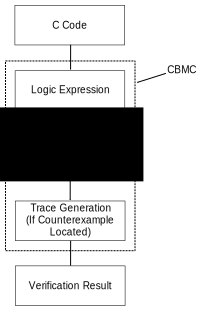
\includegraphics{formal/cbmc}}
\caption{CBMC Processing Flow}
\label{fig:formal:CBMC Processing Flow}
\end{figure}

In addition, front-end programs for SAT solvers can automatically translate
C code into logic expressions, taking assertions into account and generating
assertions for error conditions such as array-bounds errors.
One example is the C bounded model checker, or \co{cbmc}, which is
available as part of many Linux distributions.
This tool is quite easy to use, with \co{cbmc test.c} sufficing to
validate \path{test.c}, resulting in the processing flow shown in
Figure~\ref{fig:formal:CBMC Processing Flow}.
This ease of use is exceedingly important because it opens the door
to formal verification being incorporated into regression-testing
frameworks.
In contrast, the traditional tools that require non-trivial translation
to a special-purpose language are confined to design-time verification.

More recently, SAT solvers have appeared that handle parallel code.
These solvers operate by converting the input code into single static
assignment (SSA) form, then generating all permitted access orders.
This approach seems promising, but it remains to be seen how well
it works in practice.
One encouraging sign is work in 2016 applying \co{cbmc} to Linux-kernel
RCU~\cite{LihaoLiang2016VerifyTreeRCU,Liang:2018:VTB,LanceRoy2017CBMC-SRCU}.
This work used minimal configurations of RCU, and verified scenarios
using small numbers of threads, but nevertheless successfully ingested
Linux-kernel C code and produced a useful result.
The logic expressions generated from the C code had up to 90~million
variables, 450~million clauses, occupied tens of gigabytes of memory,
and required up to 80~hours of CPU time for the SAT solver to produce
the correct result.

Nevertheless, a Linux-kernel hacker might be justified in feeling skeptical
of a claim that his or her code had been automatically verified, and
such hackers would find many fellow skeptics going back
decades~\cite{DeMillo:1979:SPP:359104.359106}.
One way to productively express such skepticism is to provide bug-injected
versions of the allegedly verified code.
If the formal-verification tool finds all the injected bugs, our hacker
might gain more confidence in the tool's capabilities.
Of course, tools that find valid bugs of which the hacker was not yet aware
will likely engender even more confidence.
And this is exactly why there is a \co{git} archive with a 20-branch set
of mutations, with each branch potentially containing a bug injected
into Linux-kernel RCU~\cite{PaulEMcKenney2017VerificationChallenge6}.
Anyone with a formal-verification tool is cordially invited to try that
tool out on this set of verification challenges.

Currently, \co{cbmc} is able to find a number of injected bugs,
however, it has not yet been able to locate a bug that RCU's
maintainer was not already aware of.
Nevertheless, there is some reason to hope that SAT solvers will someday
be useful for finding concurrency bugs in parallel code.

% formal/stateless.tex
% SPDX-License-Identifier: CC-BY-SA-3.0

\section{Stateless Model Checkers}
\label{sec:formal:Stateless Model Checkers}

The SAT-solver approaches described in the previous section are quite
convenient and powerful, but the full tracking of all possible
executions, including state, can incur substantial overhead.
In fact, the memory and CPU-time overheads can sharply limit the size
of programs that can be feasibly verified, which raises the question
of whether less-exact approaches might find bugs in larger programs.

\begin{figure}[tbp]
\centering
\resizebox{2.1in}{!}{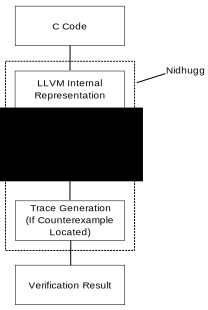
\includegraphics{formal/nidhugg}}
\caption{Nidhugg Processing Flow}
\label{fig:formal:Nidhugg Processing Flow}
\end{figure}

Although the jury is still out on this question, stateless model
checkers such as Nidhugg~\cite{CarlLeonardsson2014Nidhugg} have in
some cases handled larger programs~\cite{SMC-TreeRCU}, and with
similar ease of use, as illustrated by
Figure~\ref{fig:formal:Nidhugg Processing Flow}.
In addition, Nidhugg was more than an order of magnitude faster than
was \co{cbmc} for some Linux-kernel RCU verification scenarios.
Of course, Nidhugg's speed and scalability advantages are tied to
the fact that it does not handle data non-determinism, but this
was not a factor in these particular verification scenarios.

Nevertheless, as with \co{cbmc}, Nidhugg has not yet been able to
locate a bug that Linux-kernel RCU's maintainer was not already
aware of.
However, it was able to demonstrate that one historical bug in
Linux-kernel RCU was fixed by a different commit than the maintainer
thought, which gives some additional hope that stateless model checkers
like Nidhugg might someday be useful for finding concurrency bugs in
parallel code.


\section{Summary}
\label{sec:formal:Summary}
%
\epigraph{Western thought has focused on True-False;
	  it is high time to shift to Robust-Fragile.}
	 {\emph{summarized from Nassim Nicholas Taleb}}
% Full quote:
% Since Plato, Western thought and the theory of knowledge has focused on
% the notions of True-False; as commendable as that was, it is high time
% to shift the concern to Robust-Fragile, and social epistemology to the
% more serious problem of Sucker-Nonsucker.

The formal-verification techniques described in this chapter
are very powerful tools for validating small
parallel algorithms, but they should not be the only tools in your toolbox.
Despite decades of focus on formal verification, testing remains the
validation workhorse for large parallel software
systems~\cite{JonathanCorbet2006lockdep,DaveJones2011Trinity,PaulEMcKenney2016Formal}.

It is nevertheless quite possible that this will not always be the case.
To see this, consider that there is estimated to be more than twenty
billion instances of the Linux kernel as of 2017.
Suppose that the Linux kernel has a bug that manifests on average every million
years of runtime.
As noted at the end of the preceding chapter, this bug will be appearing
more than 50 times \emph{per day} across the installed base.
But the fact remains that most formal validation techniques can be used
only on very small codebases.
So what is a concurrency coder to do?

One approach is to think in terms of finding the first bug, the first
relevant bug, the last relevant bug, and the last bug.

The first bug is normally found via inspection or compiler diagnostics.
Although the increasingly sophisticated diagnostics provided by modern
compilers might be considered to be a lightweight sort of formal
verification, it is not common to think of them in those terms.
This is in part due to an odd practitioner prejudice which says
``If I am using it, it cannot be formal verification'' on the one
hand, and a large gap in sophistication between compiler
diagnostics and verification research on the other.

Although the first relevant bug might be located via inspection or
compiler diagnostics, it is not unusual for these two steps to find
only typos and false positives.
Either way, the bulk of the relevant bugs, that is, those bugs that
might actually be encountered in production, will often be found via testing.

When testing is driven by anticipated or real use cases, it is not
uncommon for the last relevant bug to be located by testing.
This situation might motivate a complete rejection of formal verification,
however, irrelevant bugs have an annoying habit of suddenly becoming relevant
at the least convenient moment possible, courtesy of black-hat attacks.
For security-critical software, which appears to be a continually
increasing fraction of the total, there can thus be strong motivation
to find and fix the last bug.
Testing is demonstrably unable to find the last bug, so there is a
possible role for formal verification.
That is, there is such a role if and only if formal verification
proves capable of growing into it.
As this chapter has shown, current formal verification systems are
extremely limited.

\QuickQuiz{
	But shouldn't sufficiently low-level software be for all intents
	and purposes immune to being exploited by black hats?
}\QuickQuizAnswer{
	Unfortunately, no.

	At one time, Paul E. McKenny felt that Linux-kernel RCU
	was immune to such exploits, but the advent of Row Hammer
	showed him otherwise.
	After all, if the black hats can hit the system's DRAM,
	they can hit any and all low-level software, even including RCU.

	And in 2018, this possibility passed from the realm of
	theoretical speculation into the hard and fast realm of
	objective reality~\cite{McKenney:2019:CRS:3319647.3325836}.
}\QuickQuizEnd

Another approach is to consider that
formal verification is often much harder to use than is testing.
This is of course in part a cultural statement, and there is every reason
to hope that formal verification will be perceived to be easier as more
people become familiar with it.
That said, very simple test harnesses can find significant bugs in arbitrarily
large software systems.
In contrast, the effort required to apply formal verification seems to
increase dramatically as the system size increases.

I have nevertheless made occasional use of formal verification
for almost 30 years by playing to formal verification's strengths,
namely design-time verification of small complex portions of the overarching
software construct.
The larger overarching software construct is of course validated by testing.

\QuickQuiz{
	In light of the full verification of the L4 microkernel,
	isn't this limited view of formal verification just a little
	bit obsolete?
}\QuickQuizAnswer{
	Unfortunately, no.

	The first full verification of the L4 microkernel was a tour de force,
	with a large number of Ph.D.~students hand-verifying code at a
	very slow per-student rate.
	This level of effort could not be applied to most software projects
	because the rate of change is just too great.
	Furthermore, although the L4 microkernel is a large software
	artifact from the viewpoint of formal verification, it is tiny
	compared to a great number of projects, including LLVM,
	\GCC, the Linux kernel, Hadoop, MongoDB, and a great many others.
	In addition, this verification did have limits, as the researchers
	freely admit, to their credit:
	\url{https://wiki.sel4.systems/FrequentlyAskedQuestions#Does_seL4_have_zero_bugs.3F}.

	Although formal verification is finally starting to show some
	promise, including more-recent L4 verifications involving greater
	levels of automation, it currently has no chance of completely
	displacing testing in the foreseeable future.
	And although I would dearly love to be proven wrong on this point,
	please note that such proof will be in the form of a real tool
	that verifies real software, not in the form of a large body of
	rousing rhetoric.

	Perhaps someday formal verification will be used heavily for
	validation, including for what is now known as regression testing.
	Section~\ref{sec:future:Formal Regression Testing?} looks at
	what would be required to make this possibility a reality.
}\QuickQuizEnd

One final approach is to consider the following two definitions from
\cref{sec:debugging:Required Mindset}
and the consequence that they imply:

\begin{description}[itemsep=0pt,labelindent=1em]
\item[Definition:]	Bug-free programs are trivial programs.
\item[Definition:]	Reliable programs have no known bugs.
\item[Consequence:]	Any non-trivial reliable program contains at least
			one as-yet-unknown bug.
\end{description}

From this viewpoint, any advances in validation and verification can
have but two effects: (1)~An increase in the number of trivial programs or
(2)~A decrease in the number of reliable programs.
Of course, the human race's increasing reliance on multicore systems and
software provides extreme motivation for a very sharp increase in the
number of trivial programs.

However, if your code is so complex that you find yourself
relying too heavily on formal-verification
tools, you should carefully rethink your design, especially if your
formal-verification tools require your code to be hand-translated
to a special-purpose language.
For example, a complex implementation of the dynticks interface for
preemptible RCU that was presented in
Section~\ref{sec:formal:Promela Parable: dynticks and Preemptible RCU}
turned out to
have a much simpler alternative implementation, as discussed in
Section~\ref{sec:formal:Simplicity Avoids Formal Verification}.
All else being equal, a simpler implementation is much better than
a proof of correctness for a complex implementation.

And the open challenge to those working on formal verification techniques
and systems is to prove this summary wrong!
To assist in this task, Verification Challenge~6 is now
available~\cite{PaulEMcKenney2017VerificationChallenge6}.
Have at it!!!

\section{Choosing a Validation Plan}
\label{sec:formal:Choosing a Validation Plan}

What sort of validation should you use for your project?

As is often the case in software in particular and in engineering
in general, the answer is ``it depends''.

Note that neither running a test nor undertaking formal verification
will change your project.
At best, such effort have an indirect effect by locating a bug that
is later fixed.
Nevertheless, fixing a bug might prevent inconvenience, monetary loss,
property damage, or even loss of life.
Clearly, this sort of indirect effect can be extremely valuable.

Unfortunately, as we have seen, it is difficult to predict whether or
not a given validation effort will find important bugs.
It is therefore all too easy to invest too little---or even to fail
to invest at all, especially if development estimates proved overly
optimistic or budgets unexpectedly tight, conditions which almost
always come into play in real-world software projects.

The decision to nevertheless invest in validation is often forced by
experienced people with forceful personalities.
But this is no guarantee, given that other stakeholders might also
have forceful personalities.
Worse yet, these other stakeholders might bring stories of expensive
validation efforts that nevertheless allowed embarrassing bugs to
escape to the end users.
So although a scarred, grey-haired, and grouchy veteran might carry
the day, a more organized approach would perhaps be more useful.

Fortunately, there is a strictly financial analog to investments in
validation, and that is the insurance policy.

\IfTwoColumn{
\begin{figure*}[tb]
\centering
\resizebox{6in}{!}{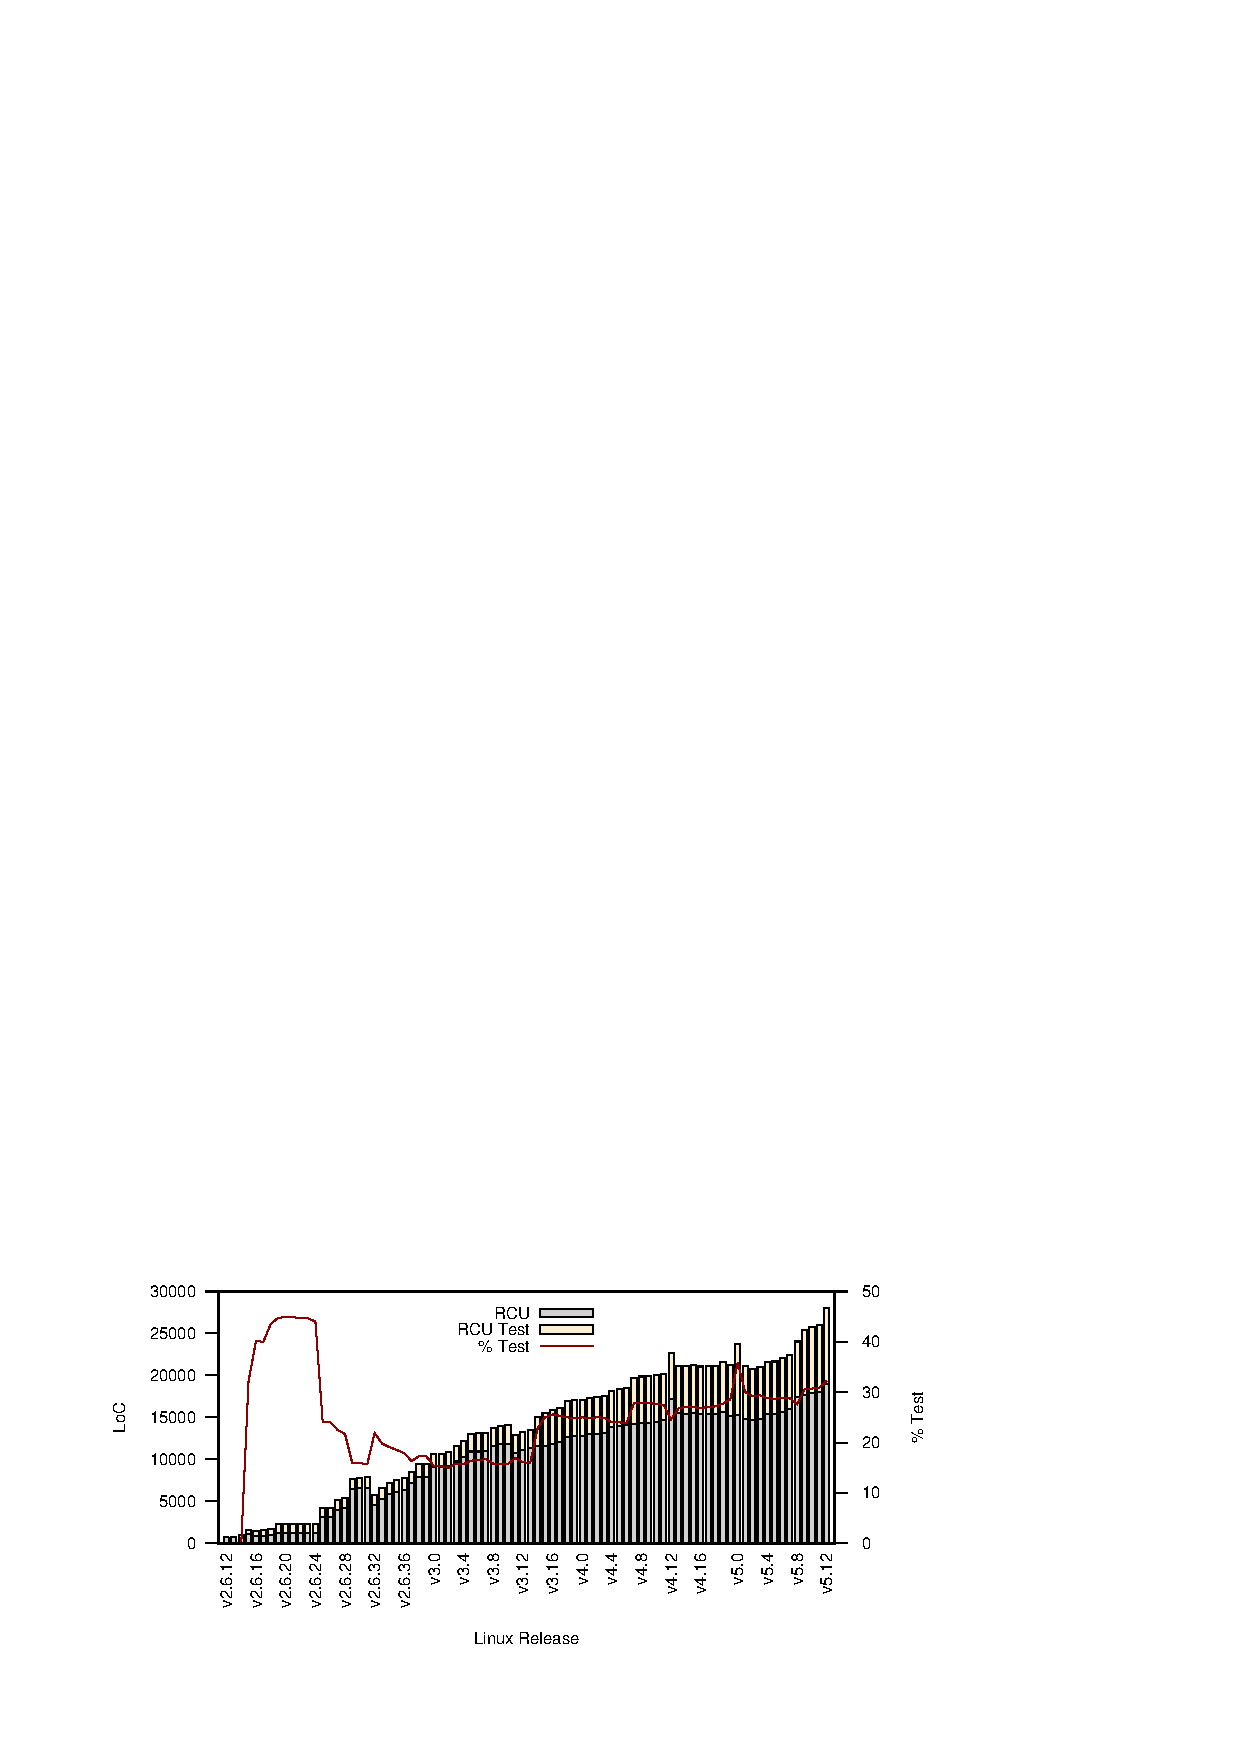
\includegraphics{formal/RCU-test-ratio.pdf}}
\caption{Linux-Kernel RCU Test Code}
\label{fig:formal:Linux-Kernel RCU Test Code}
\end{figure*}
}{}

Both insurance policies and validation efforts require consistent
up-front investments, and both defend against disasters that might
or might not ever happen.
Furthermore, both have exclusions of various types.
For example, insurance policies for coastal areas might exclude
damages due to tidal waves, while on the other hand we have seen
that there is not yet any validation methodology that can find
each and every bug.

In addition, it is possible to over-invest in both insurance and
in validation.
For but one example, a validation plan that consumed the entire
development budget would be just as pointless as would an insurance
policy that covered the Sun going nova.

One approach is to devote a given fraction of the software budget to
validation, with that fraction depending on the criticality of the
software, so that safety-critical avionics software might grant a
larger fraction of its budget to validation than would a homework
assignment.
Where available, experience from prior similar projects should be
brought to bear.
However, it is necessary to structure the project so that the validation
investment starts when the project does, otherwise the inevitable overruns
in spending on coding will crowd out the validation effort.

Staffing start-up projects with experienced people can result in
overinvestment in validation efforts.
Just as it is possible to go broke buying too much insurance, it is
possible to kill a project by investing too much in testing.
This is especially the case for first-of-a-kind projects where it is
not yet clear which use cases will be important, in which case testing
for all possible use cases will be a possibly fatal waste of time,
energy, and funding.

However, as the tasks supported by a start-up project become more routine,
users often become less forgiving of failures, thus increasing the need
for validation.
Managing this shift in investment can be extremely challenging,
especially in the all-too-common case where the users are unwilling
or unable to disclose the exact nature of their use case.
It then becomes critically important to reverse-engineer the
use cases from bug reports and from discussions with the users.
As these use cases are better understood, use of continuous integration
can help reduce the cost of finding and fixing any bugs located.

\IfTwoColumn{}{
\begin{figure}[tb]
\centering
\resizebox{4.5in}{!}{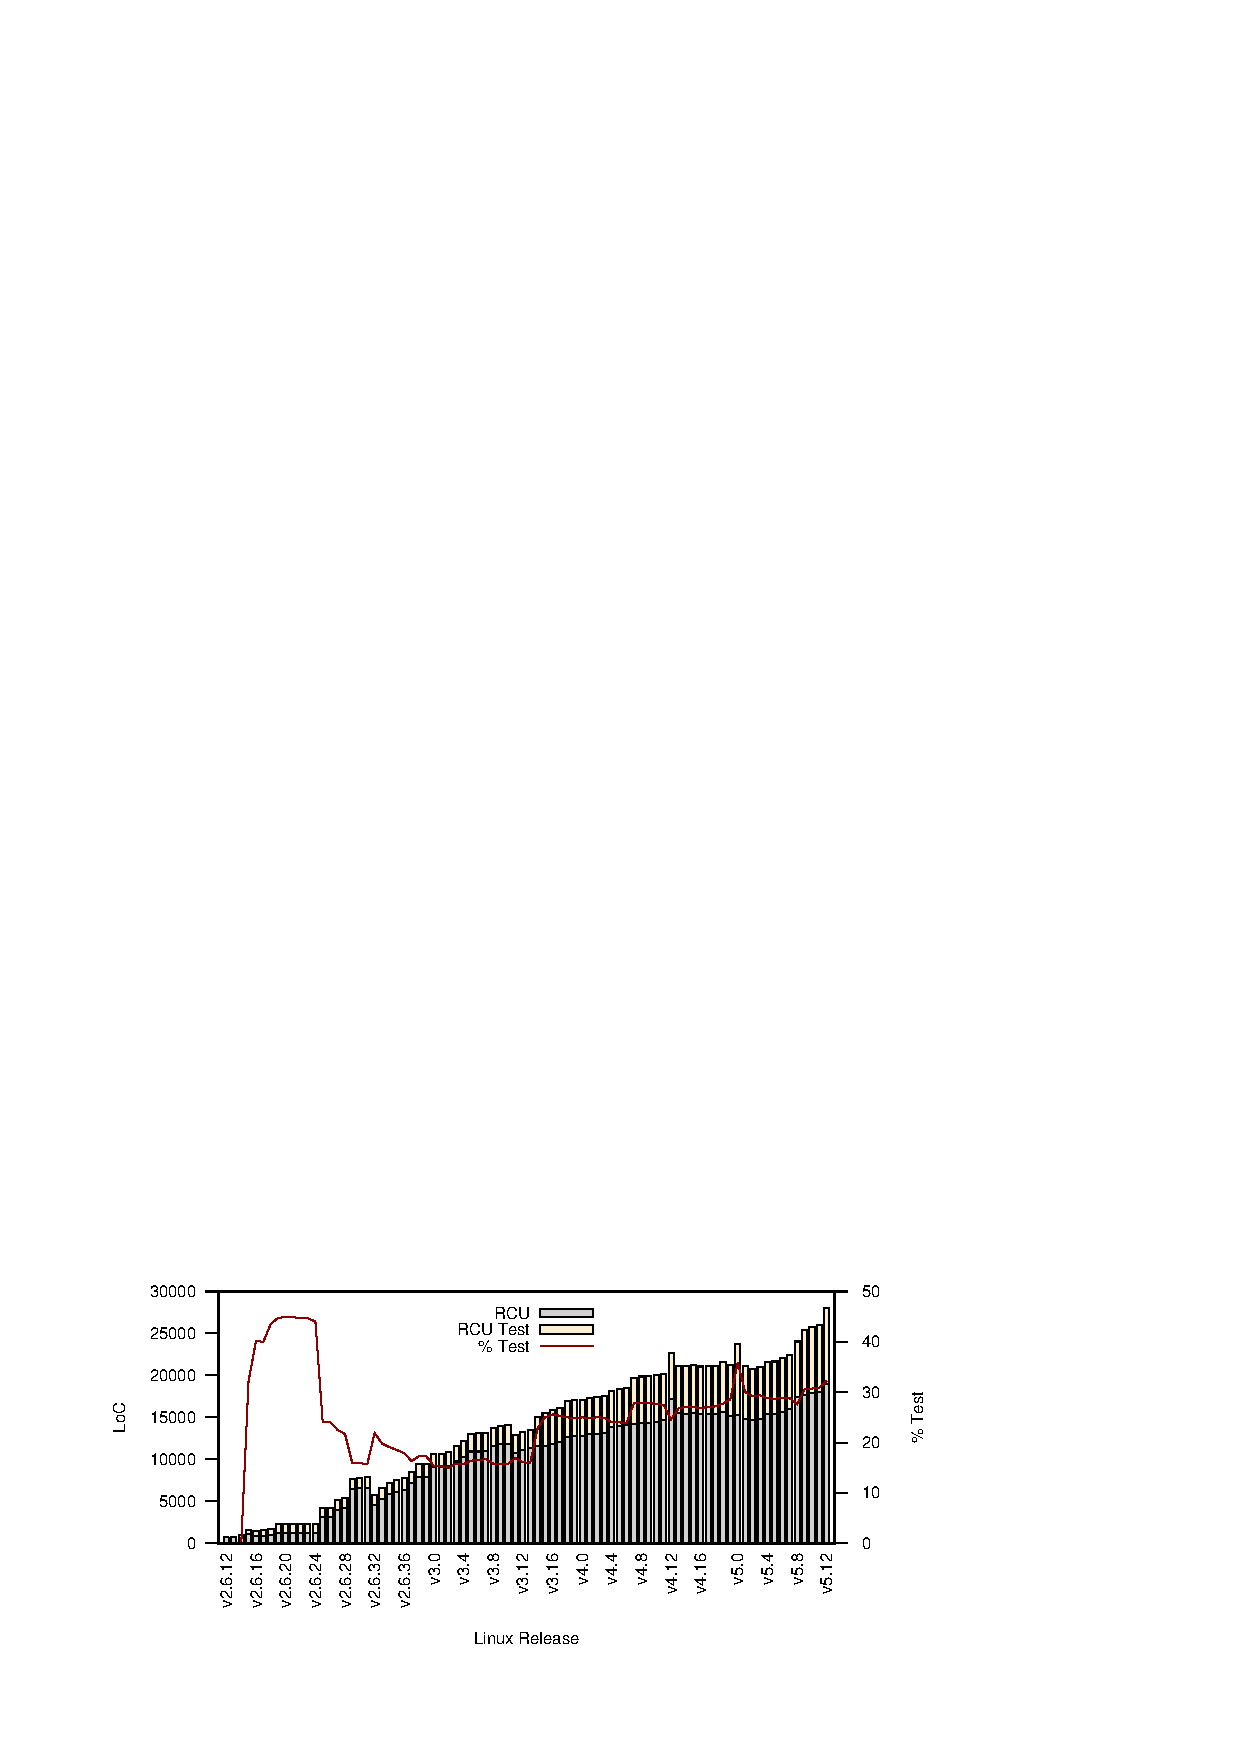
\includegraphics{formal/RCU-test-ratio.pdf}}
\caption{Linux-Kernel RCU Test Code}
\label{fig:formal:Linux-Kernel RCU Test Code}
\end{figure}
}

One example evolution of a software project's use of validation is
shown in
\cref{fig:formal:Linux-Kernel RCU Test Code}.
As can be seen in the \lcnamecref{fig:formal:Linux-Kernel RCU Test Code},
Linux-kernel RCU didn't have any validation code whatsoever until Linux
kernel v2.6.15, which was released more than two years after RCU was
accepted into the kernel.
The test suite achieved its peak fraction of the total lines of code
in Linux kernel v2.6.19--v2.6.21.
This fraction decreased sharply with the acceptance of preemptible RCU
for real-time applications in v2.6.25.
This decrease was due to the fact that the RCU API was identical
in the preemptible and non-preemptible variants of RCU.
This in turn meant that the existing test suite applied to both variants,
so that even though the Linux-kernel RCU code expanded significantly,
there was no need to expand the tests.

Subsequent bars in \cref{fig:formal:Linux-Kernel RCU Test Code} show
that the RCU code base expanded significantly, but that the
corresponding validation code expanded even more dramatically.
Linux kernel v3.5 added tests for the \co{rcu_barrier()} API, closing
a long-standing hole in test coverage.
Linux kernel v3.14 added automated testing and analysis of test results,
moving RCU towards continuous integration.
Linux kernel v4.7 added a performance validation suite for RCU's update-side
primitives.
Linux kernel v4.12 added Tree SRCU, featuring improved update-side
scalability, and v4.13 removed the old less-scalable SRCU implementation.
Linux kernel v5.0 briefly hosted the \path{nolibc} library within
the rcutorture scripting directory before it moved to its long-term
home in \path{tools/include/nolibc}.
Linux kernel v5.8 added the Tasks Trace and Rude flavors of RCU.
Linux kernel v5.9 added the \path{refscale.c} suite of read-side performance
tests.
Numerous other changes may be found in the Linux kernel's \co{git} archives.
% rcutorture
% v2.6.15: First torture test
% v2.6.19: SRCU: Plugin architecture avoids test-code explosion.
% v2.6.19-21: Peak test fraction.
% v2.6.25: preemptible RCU, consistent API avoids added test code.
% v3.4: Add tests for RCU CPU stall warnings.
% v3.5: Add tests for rcu_barrier(). *
% v3.14: Add rcutorture scripting automating tests and results analysis. *
% v3.15: Add support for multiple torture-tests suites for locktorture.
% v3.16: Add support for conditional grace-period primitives.
% v4.7: Add update-side performance validation suite. *
% v4.12: Added Tree SRCU.
% v4.13: Removed non-Tree SRCU.
% v5.0: nolibc was briefly in the rcutorture scripting directory.
% v5.8: Added Tasks Trace RCU and Rude RCU.
% v5.9: Added refscale.c.

We have established that the validation budget varies from one project
to the next, and also over the lifetime of any given project.
But how should the validation investment be split between testing and
formal verification?

This question is being answered naturally as compilers adopt increasingly
aggressive formal-verification techniques into their diagnostics and
as formal-verification tools continue to mature.
In addition, the Linux-kernel lockdep and KCSAN tools illustrate the
advantages of combining formal verification techniques with run-time
analysis, as discussed in \cref{sec:debugging:Assertions}.
Other combined techniques analyze traces gathered from
executions~\cite{DanielBristot2019RTtrace}.
For the time being, the best practice is to focus first on testing and to
reserve explicit work on formal verification for those portions of the
project that are not well-served by testing, and that have exceptional
needs for robustness.
For example, Linux-kernel RCU relies primarily on testing, but has
made occasional use of formal verification as discussed in this chapter.

In short, choosing a validation plan for concurrent software remains
more an art than a science, let alone a field of engineering.
However, there is every reason to expect that increasingly rigorous
approaches will continue to become more prevalent.

\QuickQuizAnswersChp{qqzformal}
